\chapter{Improving Model Generalization Performance}
\label{chapter:experiments2}

This chapter is divided into three different sections which will address the problems left open in \Cref{chapter:experiments}, namely, the low generalization performance on the validation and test sets in comparison to the training set. For this purpose, \Cref{section:balance} studies the impact of dataset size, data augmentation methods, and class balancing techniques. Subsequently, \Cref{section:ensemble} attempts to improve this approach's performance by finding a suitable way for ensembling multiple models from different architectures. Afterward, \Cref{section:outdist} presents results of different procedures to deal with the out of the training distribution test images. Finally, \Cref{section:discussion} discusses and compares the obtained results to other state-of-the-art skin lesion diagnosis classifiers from the \ac{ISIC} 2019 challenge. \par 

\section{Data Study} \label{section:balance}
    This section will explore the influence of factors like dataset size, data augmentation, and class balancing in the overall generalization capability of different variants of DenseNet pre-trained models. For each experiment, a benchmark has been set taken into consideration the results obtained in \Cref{chapter:experiments}. More specifically:
    \begin{itemize}
        \item Pre-trained models from the DenseNet architecture will be used, as they are part of one of the best performing architectures in this dataset (see \autoref{fig:pre_trained_model_val_comp}), while also having a comparatively small number of trainable parameters for all of its 3 tested variants, namely, the DenseNet121, DenseNet169, DenseNet201 (see \autoref{tables:pretrainedmodels});
        \item An global average pooling layer is introduced at the end of the convolutional base in order to reduce the number of parameters for the classifier;
        \item The original pre-trained model's classifier is replaced by a new classifier composed of one fully-connected layer with 512 neurons which use the ReLU activation function, and one softmax layer with 8 neurons to translate each of the class's probabilities;
        \item For the transfer learning approach, all the layer's parameters from the convolutional base of the pre-trained model are extracted and fine-tuned, which yields the best performance for the \ac{ISIC} 2019 dataset (see the results presented in \Cref{section:models});
        \item Following the work done by Gessert \textit{et al.} \cite{gessert2018} the Adam optimizer \cite{adam} is used, with $\rho_{1} = 0.9$ and $\rho_{2}=0.999$;
        \item The convolutional base is frozen for the initial 2 epochs with a learning rate of $10^{-3}$. The initial fine-tuning learning rate is $10^{-4}$, but is reduced by a factor of 10 when validation loss stops improving for 8 epochs. Each model trains for a maximum of 100 epochs but early stopping is performed whenever validation loss stops improving for 16 epochs;
        \item For each epoch, all the samples are shuffled before being feed into the network;
        \item Each batch is composed of 8 samples;
        \item For each training process, 3 models are saved: The model that obtained the highest \ac{BMA} on the validation set, the model with the lowest loss on the validation set, and finally the resulting model from the last epoch. However, the performance on the test set is evaluated according to the model which attained the highest \ac{BMA} on the validation set. 
    \end{itemize}
    
    \subsection{Impact of Dataset Size}
    \label{section:dataset_impact}
    DenseNet201 has a considerably large number of trainable parameters when compared with other models such as DenseNet121 (see \autoref{tables:pretrainedmodels}), which in theory means that it is easier for the model to memorize samples, and therefore overfit. As such, by lowering the capacity of the network, one will force it to learn more generalizable patterns within the training data. To put this into test, results for variations of the DenseNet with a smaller number of parameters, specifically, DenseNet121 and DenseNet169, were compared with DenseNet201 in \autoref{fig:densenet_variations_5000_comp}. Results show that indeed lowering the network's capacity reduces the amount of overfitting, but not by a significant margin.
    \begin{figure}[ht]
        \centering
        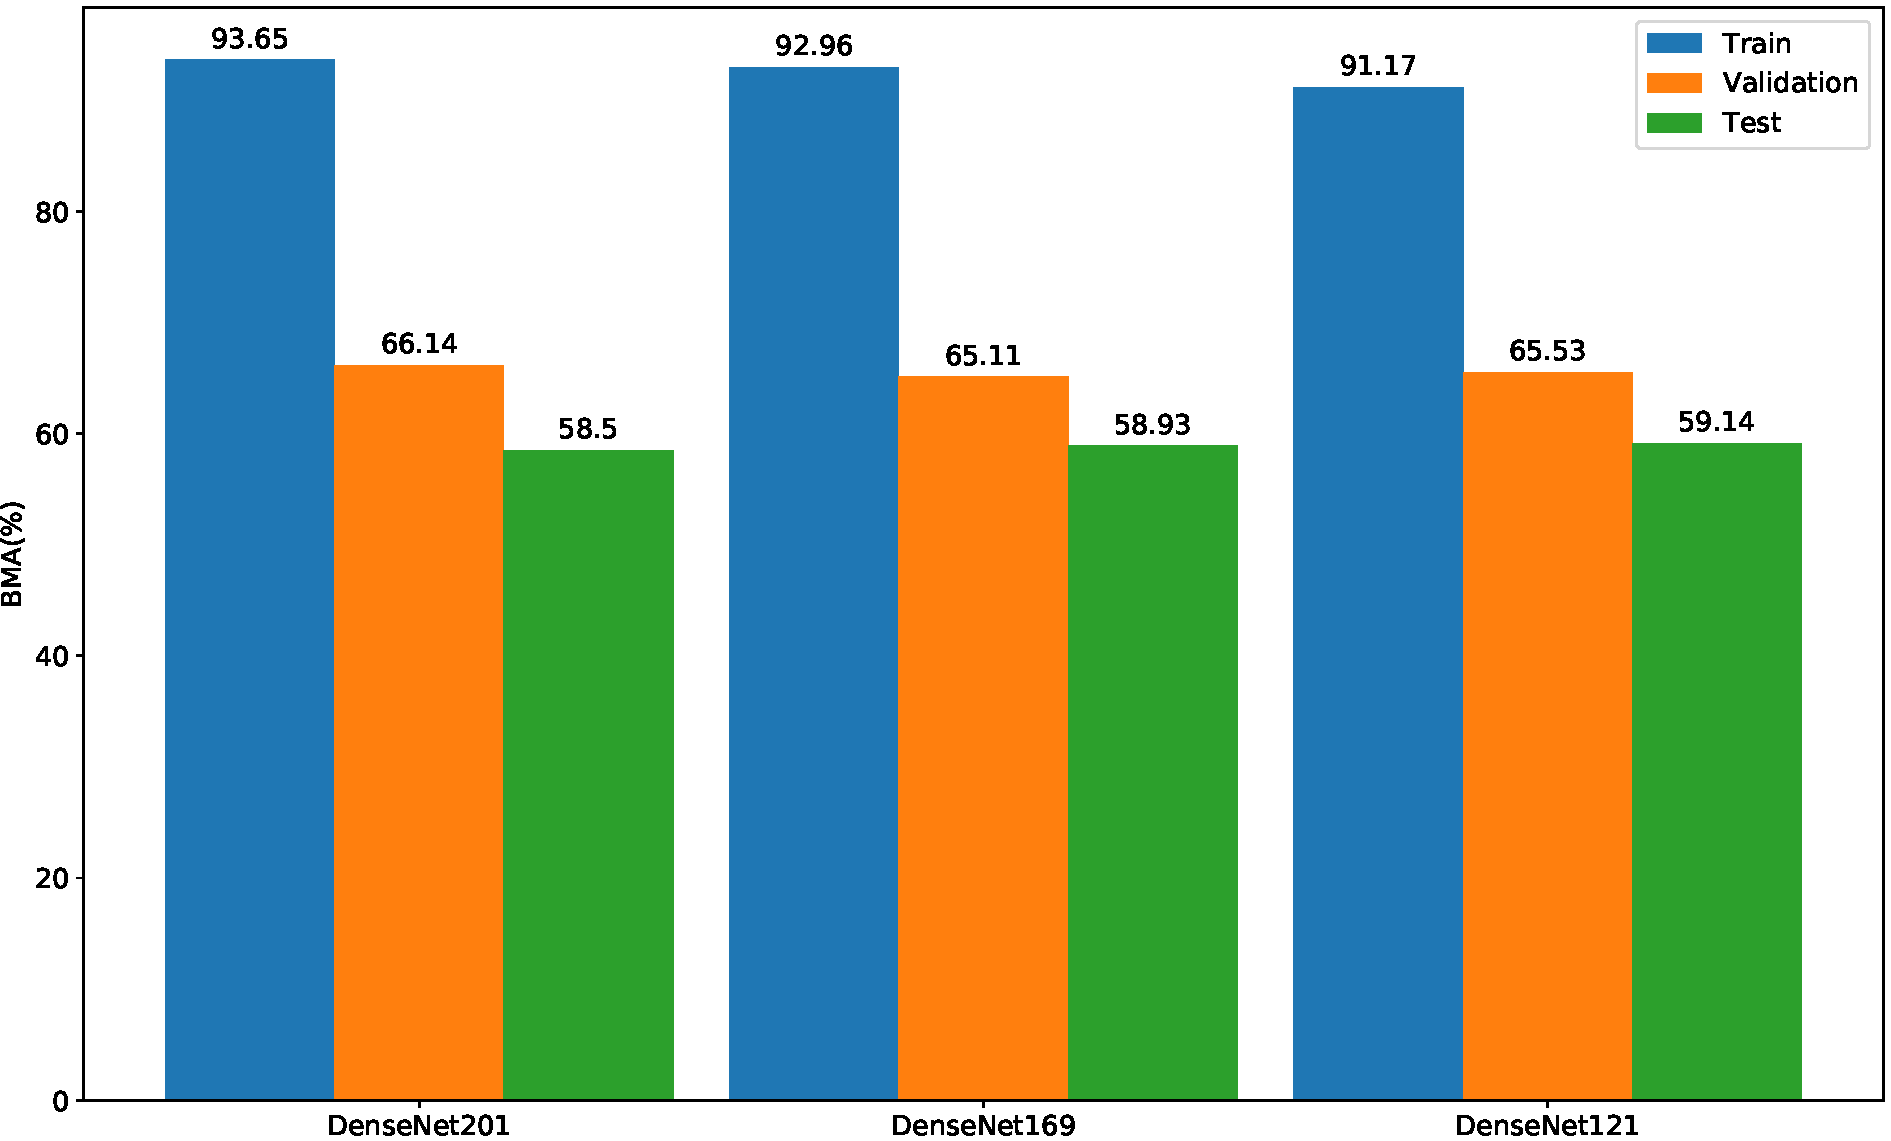
\includegraphics[width=0.9\textwidth]{figs/densenet_variations_5000_comp_2.pdf}
        \caption[Different hyperparameter tuned DenseNet pre-trained models trained with 5000 samples vs \ac{BMA} on train, validation and test sets.]{Different hyperparameter tuned DenseNet pre-trained models trained with 5000 samples vs \ac{BMA} on train, validation and test sets. Online data augmentation is turned on.}
        \label{fig:densenet_variations_5000_comp}
    \end{figure}
    
    Moreover, the DenseNet121 model in \autoref{fig:densenet_variations_5000_comp} still shows a considerable amount of overfitting, as the validation \ac{BMA} does not approximate the train \ac{BMA}. Presumably, these results stem from an inappropriate number of training samples relative to the number of free parameters in the network. The dataset used so far has been an undersampled version of the \ac{ISIC} 2019 challenge dataset, more specifically, 5000 training samples that keep the same class distribution as the original \ac{ISIC} 2019 challenge dataset. This means that underrepresented classes like dermatofibroma have too few samples to learn strong generalizable features (see \autoref{fig:distribution}). \par
    
    Indeed, the results in \autoref{fig:samples_comp} show that an increase in dataset size enables the DenseNet201 model to attain an significantly better validation \ac{BMA} score. So far, this has been the only comparison that was able to significantly improve generalization performance and reduce overfitting, corroborating the importance of the dataset used for training deep neural networks. However, it should be noted that even with the full dataset (20517 training samples), overfitting remains an issue that should be addressed. \par
    \begin{figure}[ht]
        \centering
        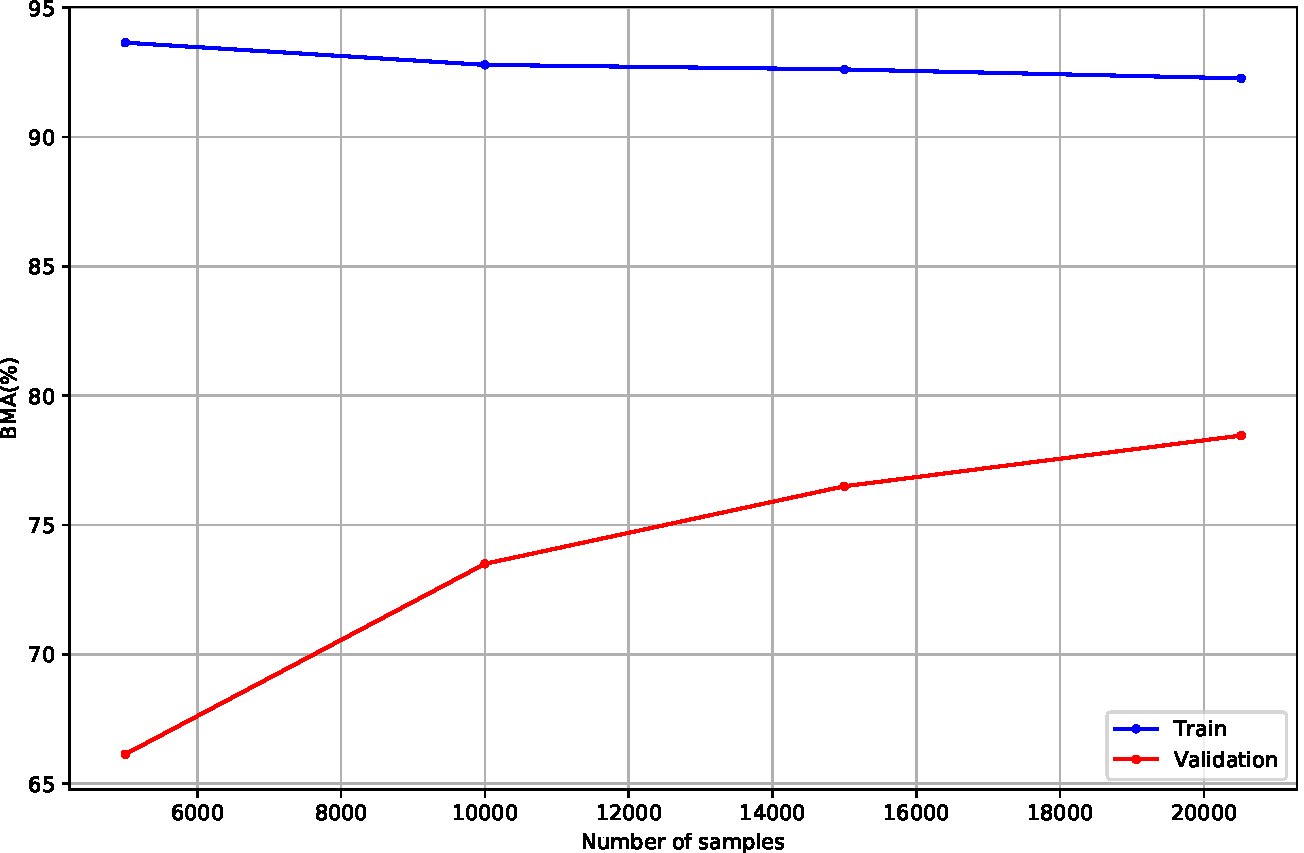
\includegraphics[width=0.8\textwidth]{figs/densenet201_samples_comp.pdf}
        \caption[Number of training samples vs train and validation \ac{BMA} for the DenseNet201 pre-trained model.]{Number of training samples vs train and validation \ac{BMA} for the DenseNet201 pre-trained model. Online data augmentation is turned on.}
        \label{fig:samples_comp}
    \end{figure}
    
    Furthermore, by observing \autoref{fig:samples_bma_over_epochs}, one can see that models trained with more samples take longer to converge. Presumably, this is related to the learning rate scheduler, because in models with more samples, validation loss keeps improving for longer with high learning rates (\textit{e.g.}, $10^{-4}$), which makes the scheduler decrease the learning rate later (see \autoref{fig:samples_lr_over_epochs}). In contrast, models trained with fewer samples stop improving the validation loss earlier, which makes the learning rate scheduler decrease the learning rate earlier. Consequently, as models tend to convergence to a local minimum with low learning rates, models trained with more samples take longer to converge because they take longer to reach low learning rates. \par
    
    \begin{figure}[ht]
        \centering
        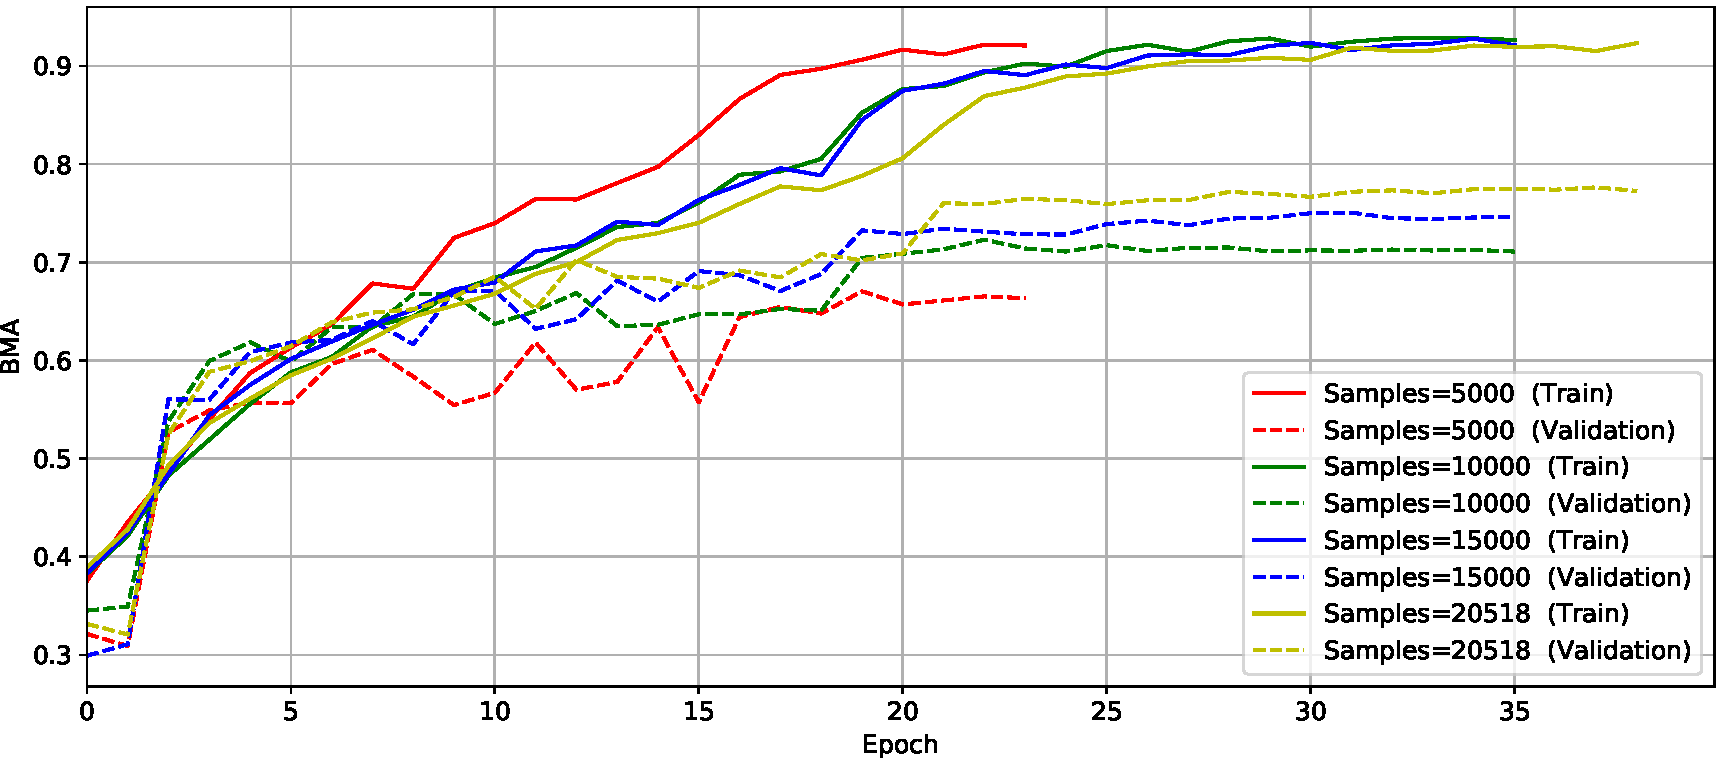
\includegraphics[width=\textwidth]{figs/densenet201_samples_bma_over_epochs.pdf}
        \caption[Number of training samples vs train and validation \ac{BMA} over epochs for the DenseNet201 model.]{Number of training samples vs train and validation \ac{BMA} over epochs for the DenseNet201 model. Online data augmentation is turned on.}
        \label{fig:samples_bma_over_epochs}
    \end{figure}
    \begin{figure}[ht]
        \centering
        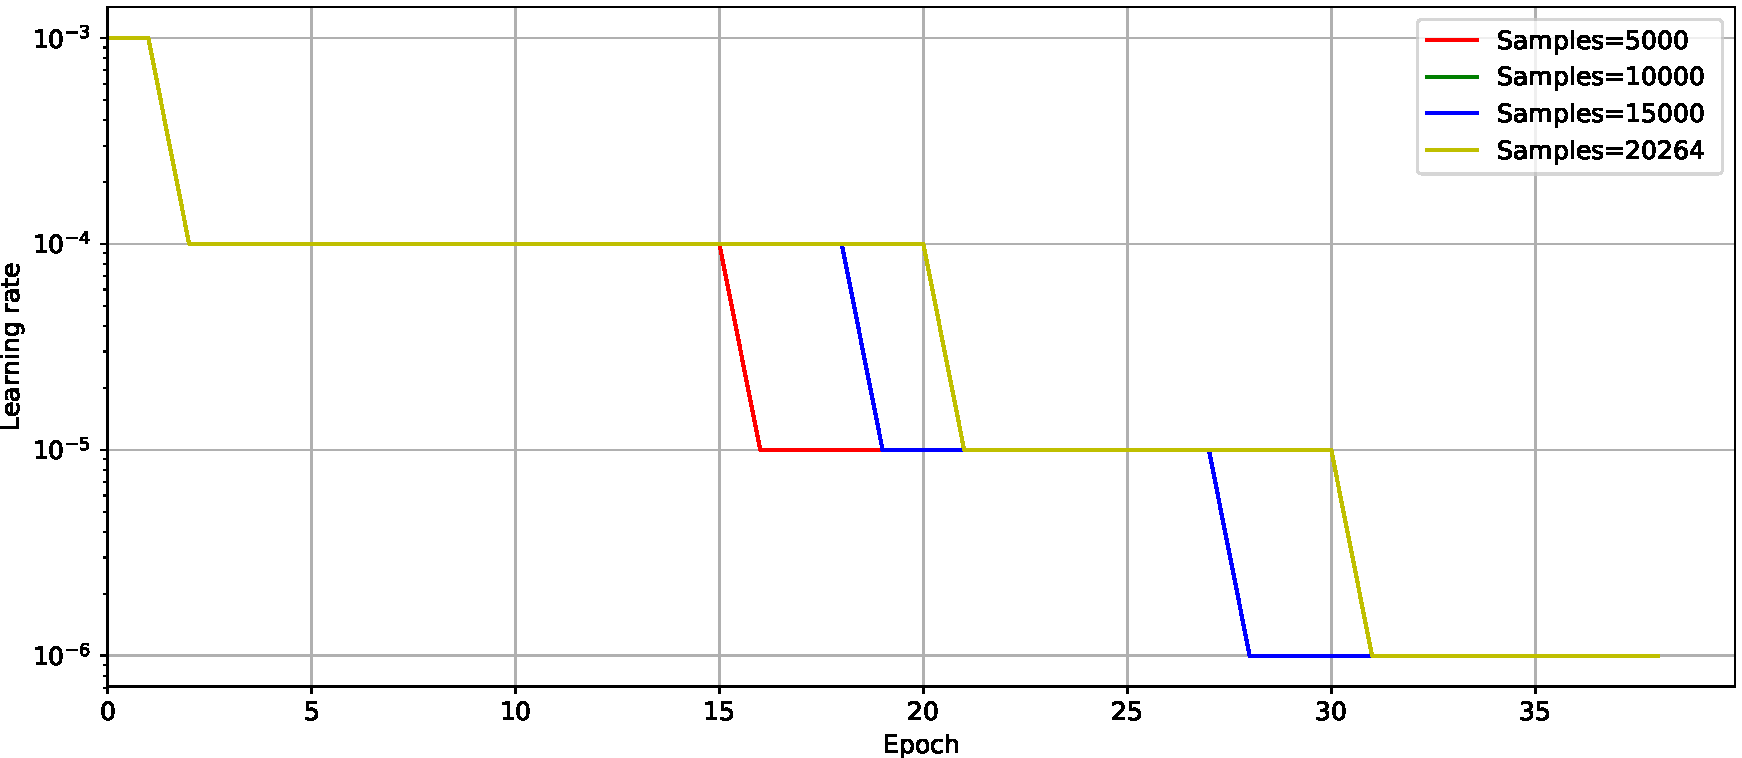
\includegraphics[width=\textwidth]{figs/densenet201_samples_lr_over_epochs.pdf}
        \caption{Influence of the number of samples on the learning rate over epochs for the DenseNet201 model.}
        \label{fig:samples_lr_over_epochs}
    \end{figure}
    
    The results from the plot graph in \autoref{fig:densenet_variations_5000_comp} show that one could use a smaller pre-trained model from DenseNet, while maintaining similar performance, which would overall be beneficial to reduce overfitting. However, with a larger dataset, one could argue that the gap between models with a high and low number of trainable parameters would increase. Therefore, an experiment with different variations of the DenseNet has been made with 20517 training samples, to assess if this hypothesis is correct. \par
    
    Nevertheless, results in \autoref{fig:densenet_variations_20264_comp} show no significant improvements between different variants of the DenseNet architecture. Even though DenseNet201 got the best performance in comparison with its smaller versions, this improvement is not substantial as the difference between the DenseNet121 and DenseNet201 on test data is about 0.08\%. Considering the results, that difference becomes even more irrelevant when taken into consideration that the \ac{BMA} gap between train and test on DenseNet121 is lower when compared with both DenseNet169 and DenseNet201. As such, the smaller model DenseNet121 proves to be a better choice as it slightly reduces overfitting while keeping similar performance to bigger models on the test set. \par
    
    \begin{figure}[ht]
        \centering
        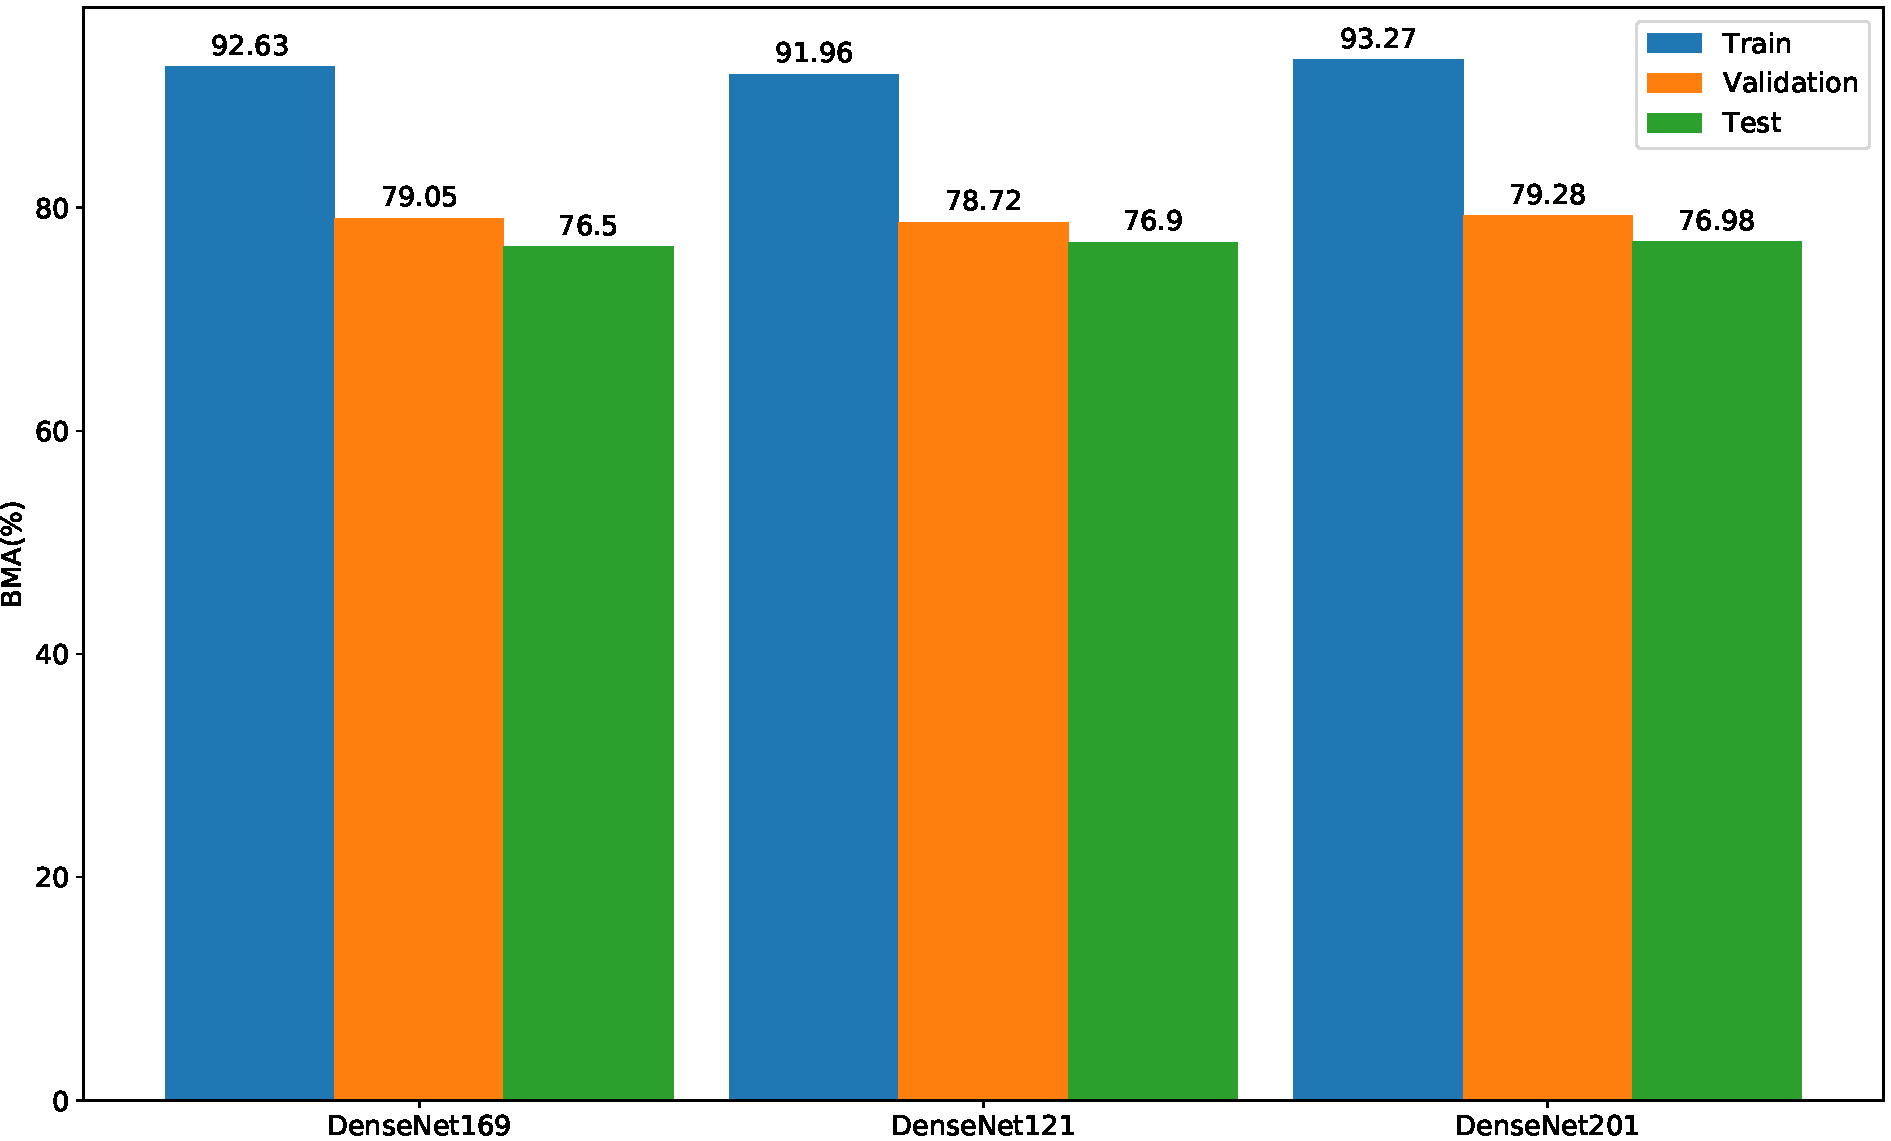
\includegraphics[width=0.9\textwidth]{figs/densenet_variations_20264_comp.pdf}
        \caption[Different hyperparameter tuned DenseNet pre-trained models trained with 20518 samples vs \ac{BMA} on train, validation and test sets]{Different hyperparameter tuned DenseNet pre-trained models trained with 20518 samples vs \ac{BMA} on train, validation and test sets. Online data augmentation is turned on.}
        \label{fig:densenet_variations_20264_comp}
    \end{figure}
    
    Finally, with the full dataset, the DenseNet121 model is able to attain a \ac{BMA} of 76.9\% and a accuracy of 84.9 \% over the test set. Furthermore, results show considerable improvements on the confusion matrix in \autoref{fig:unbalanced_full_dataset_conf_matrix} when compared with the results from \autoref{fig:hyperparameter_tuned_conf_matrix}. Overall every single class attains better performance on the test set, but this effect is much more noticeable in classes with fewer samples. Presumably, these results could be further improved with a larger training dataset, which should be a focus point for future benchmark challenges of \ac{ISIC}. \par
    
    \begin{figure}[ht]
        \centering
        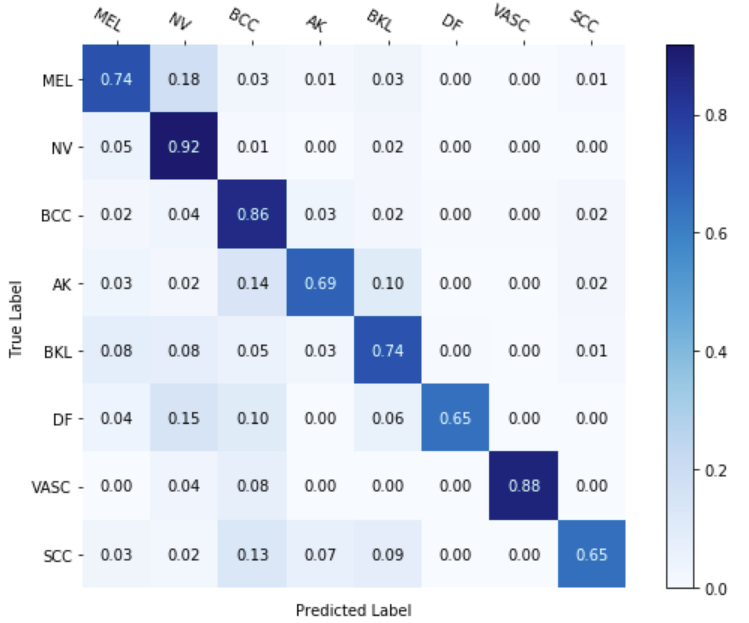
\includegraphics[width=0.7\textwidth]{figs/densenet201_20517_unbalanced_conf_matrix.png}
        \caption[Confusion matrix of the hyperparameter optimized and fine-tuned DenseNet121 pre-trained model trained with the full unbalanced training dataset.]{Confusion matrix of the hyperparameter optimized and fine-tuned DenseNet121 pre-trained model trained with the full unbalanced training dataset (20517 samples). Online data augmentation was turned on as a measure to reduce overfitting.}
        \label{fig:unbalanced_full_dataset_conf_matrix}
    \end{figure}
    
    \subsection{Impact of Augmentation Techniques}
    \label{section:dg_impact}
    Considering the results from \autoref{fig:samples_comp}, there is a considerable amount of overfitting even with the full training dataset. Moreover, results in \autoref{fig:unbalanced_full_dataset_conf_matrix}, still show a considerable lack of generalization performance for underrepresented classes. As such, different strategies of data augmentation can be used to help alleviate these problems. One of such strategies is called offline data augmentation, which attempts to create a larger dataset by generating synthetic samples through augmentation techniques before the training process starts. \par
    
    However, there is a wide range of image processing methods for augmenting images (\textit{e.g.}, rotations, distortions) and they can be combined to produce samples that are substantially different from their originals. As such, depending on the number of augmentations to be considered, there could be a huge amount of different combinations between them, especially considering that some of them have different variations and parameters which can quite change the augmentation (\textit{e.g.}, the magnitude of distortion, the angle of rotation). Therefore, it is important to determine what combinations of data augmentation techniques significantly improve the overall performance for the problem of skin lesion classification. \par
        
    Figure \ref{fig:data_aug_group_bal_acc_comp} shows a comparison between different augmentation groups applied to the DenseNet121 model trained with 20518 class balanced samples (approximately 2565 samples per class). Moreover, underrepresented classes are oversampled through the augmentation techniques from each of the groups, and overrepresented classes are undersampled by randomly choosing samples from that class without repetition. In turn, this means that 9089 samples are generated through data augmentation and the rest of the images are original (11420 samples). Furthermore, the experiments use the augmentation techniques described in \Cref{section:augmentation} which are spread across the different augmentation groups. More specifically:
    \begin{itemize}
        \item Group 0: No augmentation techniques are applied. For data augmentation as a class balancing measure (offline data augmentation), oversampling is done by randomly copying and pasting samples from a specific class with repetition. This is the baseline that other groups should be compared to;
        \item Group 1: Composed of slight variations to the original image, such as rotations of 90 degrees (clockwise), flips from top to bottom or vice versa, flips from left to right or vice versa, and crops that keep at least 85\% of the original image pixels to assure that most of the lesion stays visible;
        \item Group 2: Composed of the augmentation techniques of group 1 plus some adjustments on pixel intensities, specifically, brightness changes from 50\% to 150\% (100\% being the original image and 0\% being a black image), contrast changes from 50\% to 150\% (100\% being the original image and 0\% being a solid grey image), and coloration changes from 50\% to 150\% (100\% being the original and 0\% being a black and white image);
        \item Group 3: Composed of the augmentation techniques of group 1 plus perspective transformations. These transformations include tilts on either the left or right side, tilts forward and backward, skews from a random corner of an image, and finally, shears with a variation anywhere from 20 degrees towards the left to 20 degrees towards the right side of the image or anywhere from 20 degrees towards the top or 20 degrees towards the bottom of the image;
        \item Group 4: Composed of the augmentation techniques of group 1 plus noise induction augmentation techniques. Elastic distortions are applied with a grid size of 8, meaning that the image is divided into an 8x8 grid and each region is distorted independently. Random erasing is also applied, which takes a random area equivalent to 25\% of the original image and replaces it by random pixels, meaning that each pixel has a random intensity, ultimately producing noise in that area.
    \end{itemize}
    In groups 1, 2, 3, and 4 there is a 0.5 probability of applying a specific augmentation technique in the group augmentation pipeline, which means that the same sample augmented multiple times will likely produce different augmented samples. This is a desirable property as producing the same synthetic sample over and over again would produce a lot of repetition in highly undersampled classes. Consequently, it could lead to problems like overfitting because the network would try to minimize loss for the same repeated samples, rather than learning generalizable knowledge from variations of that sample. \par
    
    \begin{figure}[ht]
        \centering
        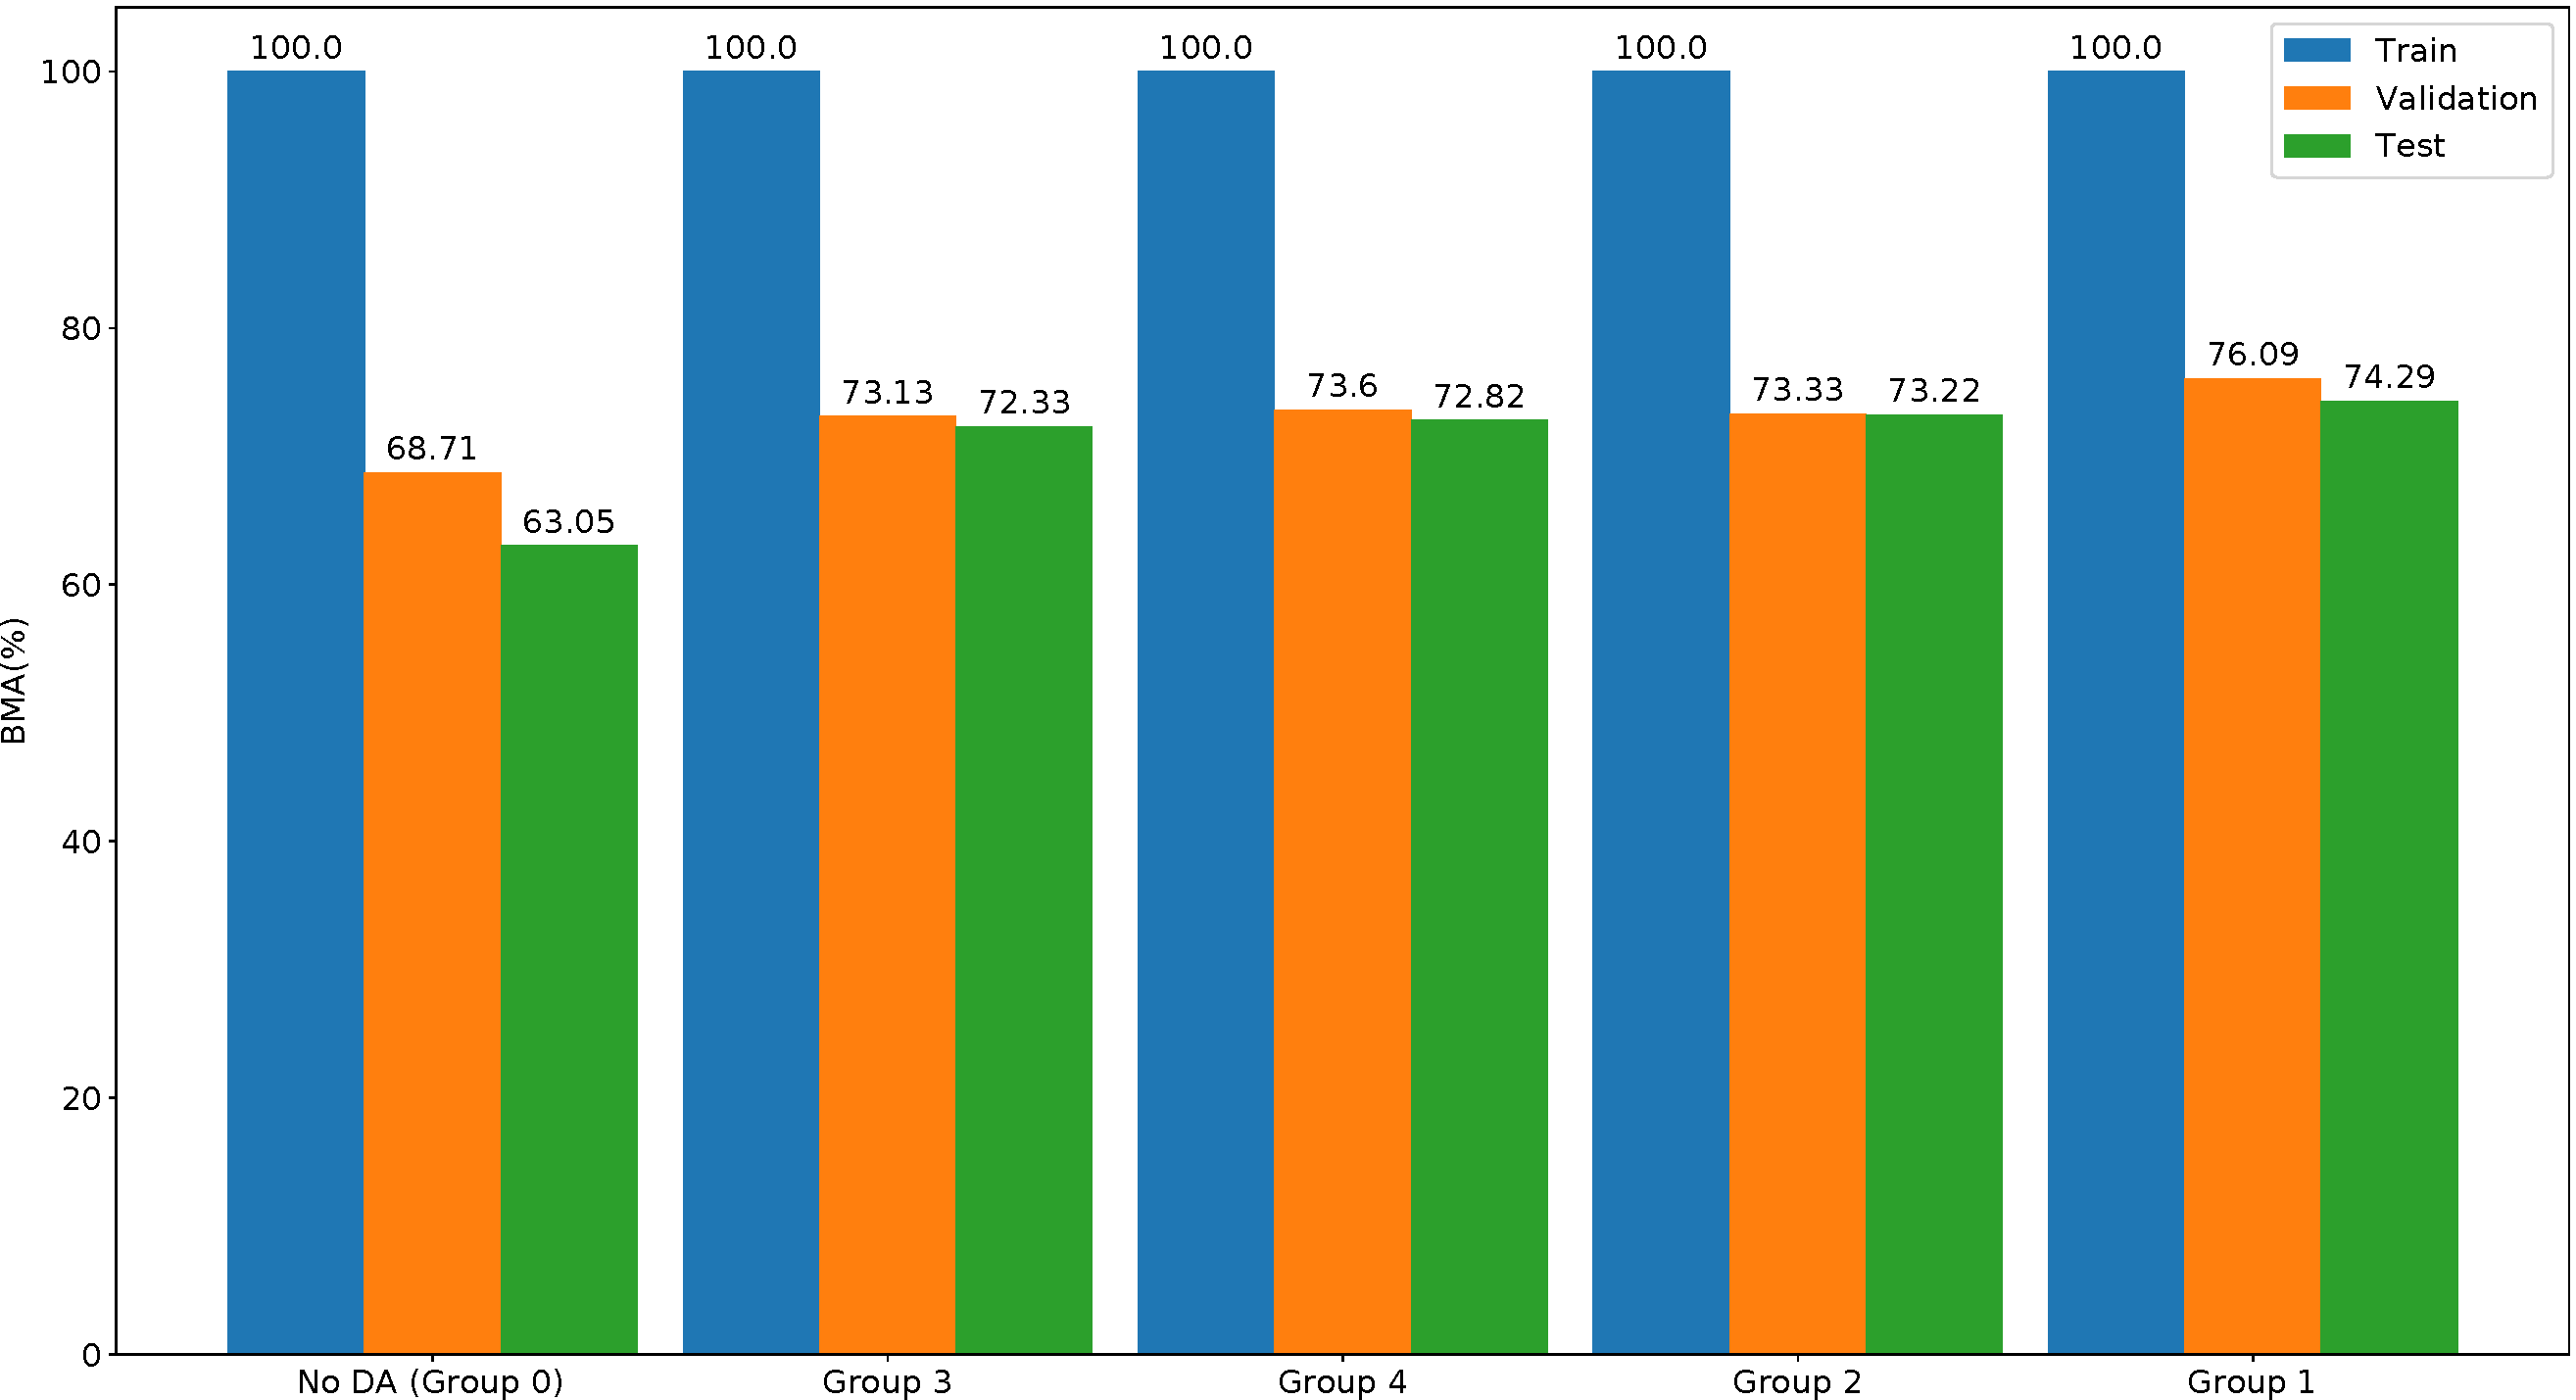
\includegraphics[width=\textwidth]{figs/data_aug_group_bal_acc_comp.pdf}
        \caption[\ac{BMA} of train, validation and test sets of different offline data augmentation groups with the DenseNet121 trained on 20518 balanced samples.]{\ac{BMA} of train, validation and test sets of different offline data augmentation groups with the DenseNet121 trained on 20518 balanced samples. Online data augmentation is turned off.}
        \label{fig:data_aug_group_bal_acc_comp}
    \end{figure}
    
    Considering the results from \autoref{fig:data_aug_group_bal_acc_comp}, overall data augmentation does improve the performance in comparison with group 0, which does not employ any type of augmentation. Moreover, results indicate that simpler augmentation techniques like group 1 and 2 perform slightly better when compared to more complex augmentations groups such as group 3 and 4, which is to be expected in the context of skin lesion classification, because such groups alter important information about the lesion itself. \par
    
    As described in \Cref{chapter:sota}, one of the methods used to identify skin lesions is the ABCDE method, which relies on features like the shape and color of the lesion to be diagnosed. Therefore, by changing such features, one is potentially removing or changing important information about the lesion itself, which consequently will make the network perform worse. For example, group 4 introduces noise inducing transformations, however, one does not have the assurance that the random erasing will not erase important information from the lesion itself. Moreover, group 4 also applies distortions in the lesion samples, but such technique can also alter the shape of the lesion in such a way that it is no longer characteristic of its original lesion type. Similarly, by changing the colors of the lesion in group 2, important information about the color of the lesion might be changed, which is often an important property used by dermatologists to diagnose a lesion (\textit{e.g.}, ABCDE method).  \par
    
    However, offline data augmentation is not the only method of applying data augmentation. Specifically, online data augmentation is from the literature presented in \Cref{chapter:sota}, a commonly used technique to reduce overfitting in deep learning based skin lesion classification models. While offline data augmentation can be used as a method to balance samples across classes, in online data augmentation, images are generated per iteration during training and differ in each epoch. In other words, in each epoch, the network is going to be fed a different variation of the original image, rather than the same image.  Moreover, the results presented in \autoref{fig:data_aug_group_bal_acc_comp} show that turning off online data augmentation will cause a huge gap between train and validation/test \ac{BMA} (overfitting), as the training \ac{BMA} is 100\% for all 5 groups. 
    
    Therefore, experiments were made to assess the impact of different combinations of online data augmentation and offline data augmentation (as a class balancing measure). As shown in \autoref{fig:data_aug_mode_bal_acc_comp}, online data augmentation significantly reduces the gap between train and validation and overall improves \ac{BMA} on the test set, both when employed with and without offline data augmentation. Even though the model with offline and online data augmentation performed better, it also increased overfitting in comparison with the model only trained with online data augmentation. Presumably, these results reflect the concerns discussed in \Cref{section:limitations}, namely, data augmentation can lead to a model that easily discriminates synthetic examples but does not generalize the attained knowledge to real data \cite{Ching2018}.  \par
    
    \begin{figure}[ht]
        \centering
        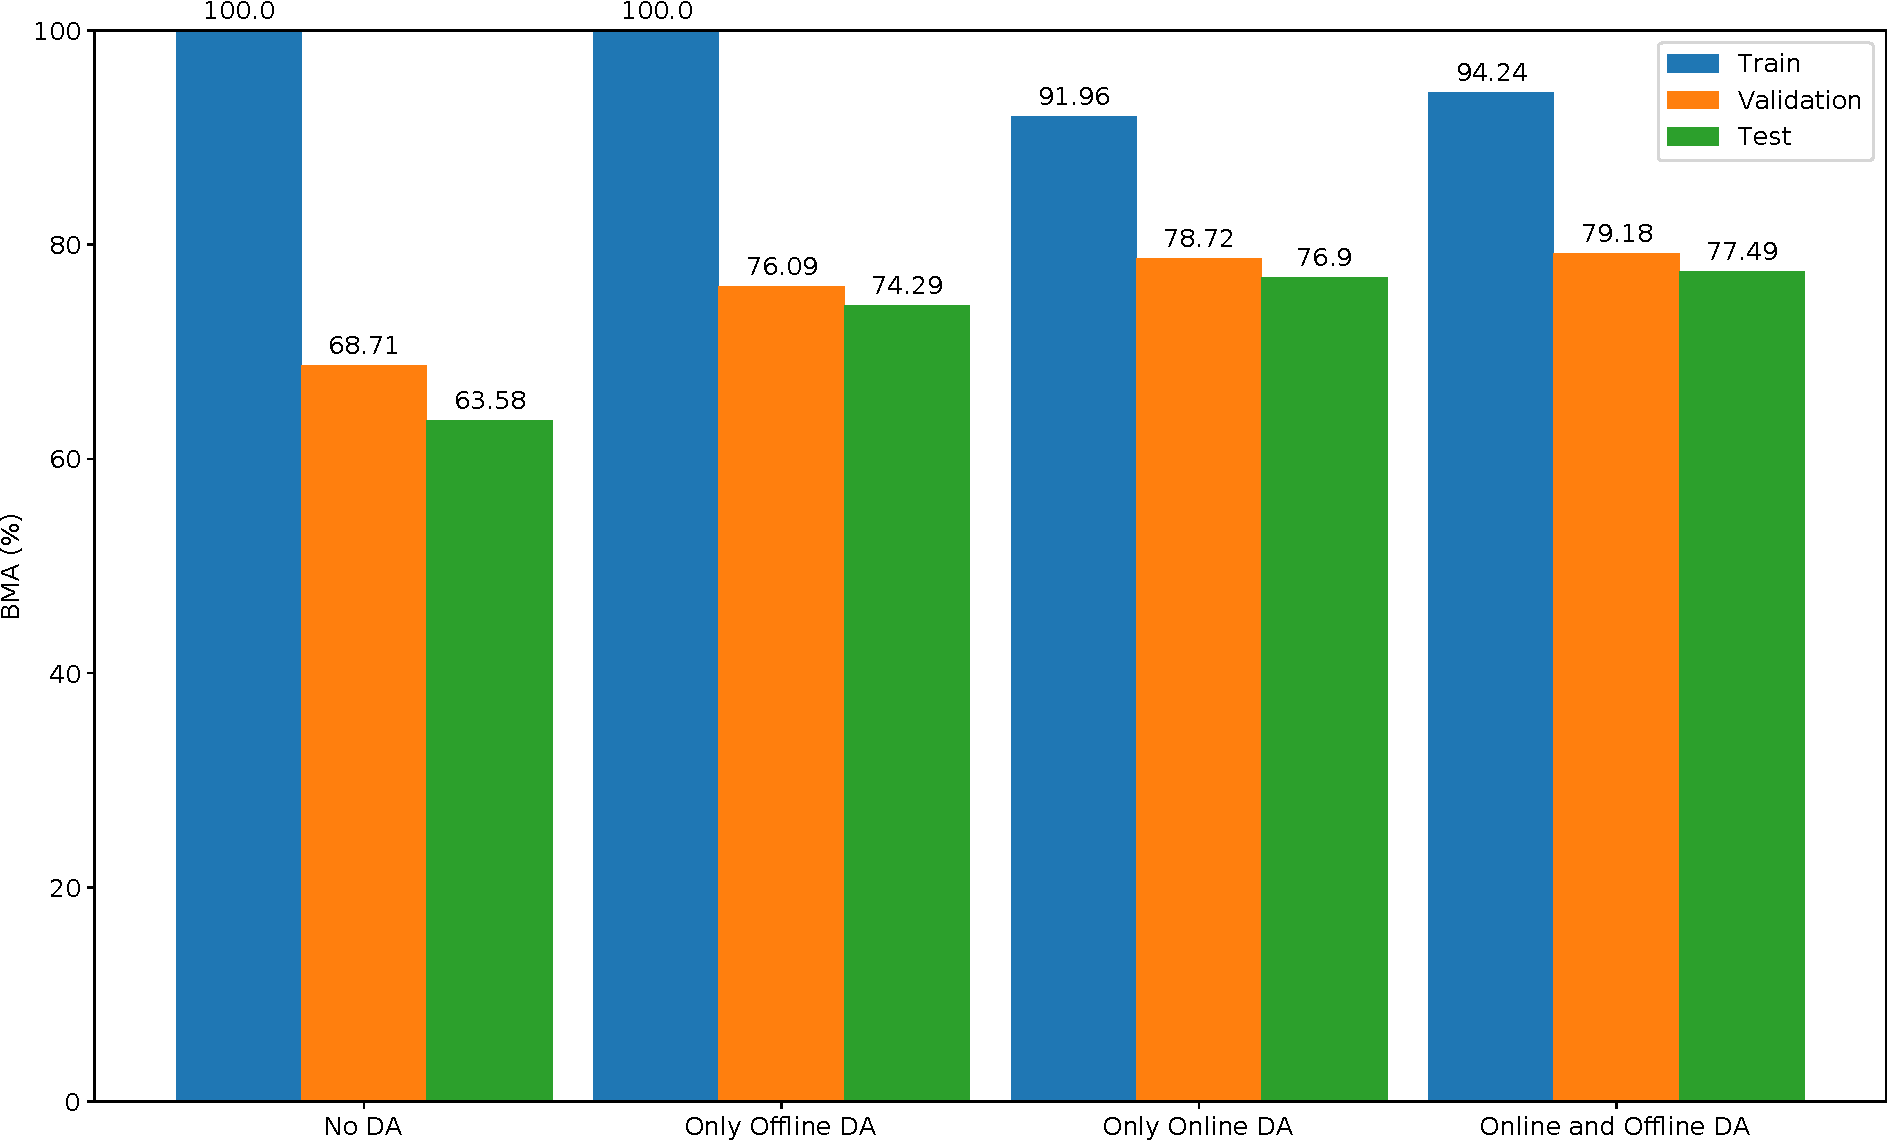
\includegraphics[width=\textwidth]{figs/data_aug_mode_bal_acc_comp.pdf}
        \caption[\ac{BMA} of the train, validation and test sets of different combinations of offline and online data augmentation modes with a hyperparameter tuned DenseNet121 trained on 20518 balanced samples.]{\ac{BMA} of the train, validation and test sets of different combinations of offline and online data augmentation modes with the DenseNet121 trained on 20518 balanced samples. "No DA" is equivalent to data augmentation group 0 and "Only Offline DA" is equivalent to group 1 in figure \autoref{fig:data_aug_group_bal_acc_comp}. "Only Online DA" simply employs online data augmentation during the training process. "Online and Offline DA" combines the class balancing measures from offline data augmentation and the overfitting measures from online data augmentation during training. }
        \label{fig:data_aug_mode_bal_acc_comp}
    \end{figure}
    
    In the experiments showed so far, online data augmentation always uses augmentation group 1, which as shown in \autoref{fig:data_aug_mode_bal_acc_comp}, significantly reduces overfitting. However, an interesting question can be made of whether other augmentation groups can have the same effect on overfitting and generalization performance for online data augmentation. As such, an experiment with different augmentation groups for online data augmentation with an unbalanced dataset has been done, where the dataset used is the original 20518 samples to not bias the obtained results (no offline data augmentation). \par
    
    \begin{figure}[ht]
        \centering
        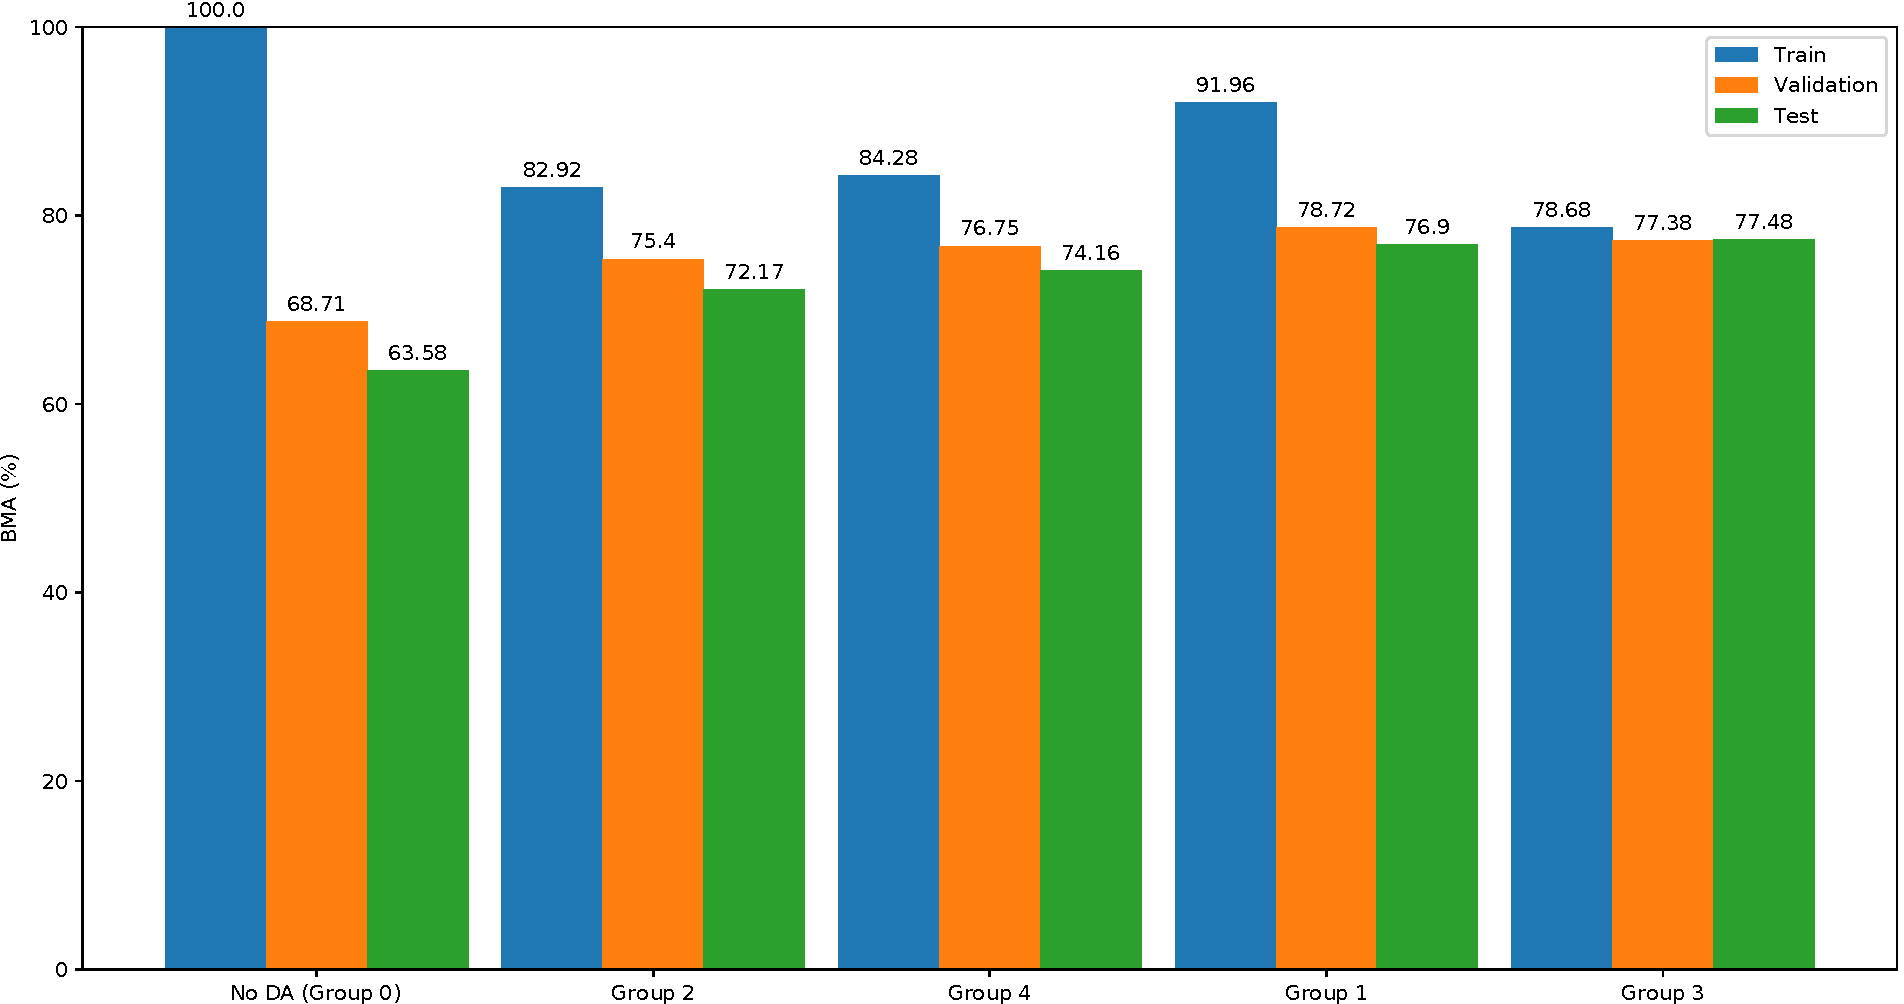
\includegraphics[width=\textwidth]{figs/data_aug_online_group_comp.pdf}
        \caption{\ac{BMA} of train, validation and test sets of different online data augmentation groups with the DenseNet121 trained on 20518 unbalanced samples (no offline data augmentation).}
        \label{fig:data_aug_online_group_comp}
    \end{figure}
    
    Figure \ref{fig:data_aug_online_group_comp} shows that online data augmentation significantly reduces overfitting for all 4 augmentation groups. Furthermore, group 3 seems to almost eliminate overfitting, because the train, validation, and test \ac{BMA} scores are quite similar. Group 3 also displays the best generalization performance on the test set in comparison with other groups. In contrast, group 1 performs slightly worse than group 3 on the test set, but significantly increases the amount of overfitting because the gap between train and validation/test is much larger. Other groups like 2 and 4 also reduce overfitting, but significantly reduce generalization performance on the test set. \par

    Presumably, these results stem from the nature of online data augmentation. Considering an input image, in each iteration of the training process, online data augmentation will produce a different image. This means that samples generated by the augmentation procedures of group 3, will produce significantly different images in each iteration of the training process (see examples in \autoref{fig:augmentations}). In contrast, group 1 will produce somewhat similar images across all iterations because it is composed of simple augmentation techniques such as flips, rotations, and crops. This means that when one uses group 3 for online data augmentation during the training process, the model is obliged to learn a different feature each time a sample is fed to the network because it sees a significantly different sample in each iteration. Therefore, the model is forced to learn generalizable knowledge across these iterations rather than memorize equal or similar samples, like in augmentation group 1. \par
    
    Unfortunately, these results came late in the development process of this work which meant that the next experiments were made using the augmentation group 1 for online data augmentation rather than group 3. Even though the \ac{BMA} scores of group 1 and 3 are similar for the test set in \autoref{fig:data_aug_online_group_comp}, the findings of using group 3 present a major way of reducing overfitting that should be further explored in future \ac{ISIC} challenges. \par 
    
    \subsection{Impact of Class Balancing through Data Augmentation}
    \label{section:class_bal_impact}
    
    The results in \autoref{fig:unbalanced_full_dataset_conf_matrix} show that even by using the full dataset, classification towards underrepresented classes (\textit{e.g.}, squamous cell carcinoma or dermatofibroma) has overall worse performance than classes with more samples (\textit{e.g.}, melanocytic nevus). Moreover, results in \autoref{fig:data_aug_group_bal_acc_comp} have shown that offline data augmentation as a class balancing measure significantly improves the \ac{BMA} scores across the train, validation and test sets. Therefore, one could hypothesize that this method can improve the generalization performance of the network further in underrepresented classes. \par
    
    Results in \autoref{fig:densenet201_bma_comp} show an experiment where a balanced model with 2533 samples per class is compared against an unbalanced model of 20518 samples by their \ac{BMA} over the train, validation, and test sets. Results show that the balanced model will attain a better \ac{BMA} score concerning all these three sets. \par
    
    \begin{figure}[ht]
        \centering
        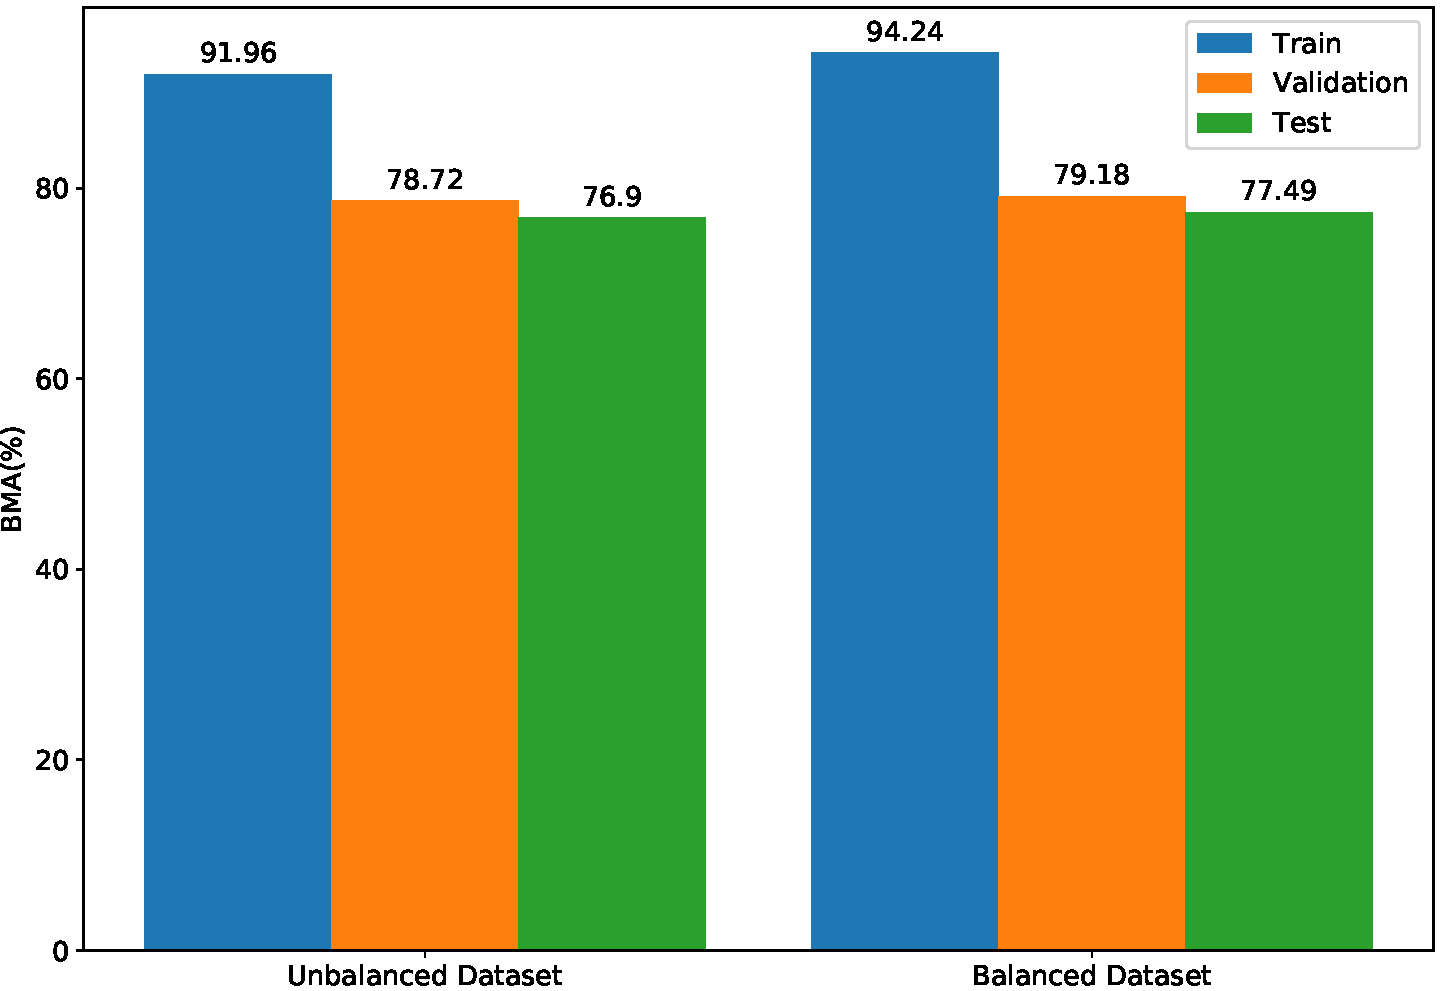
\includegraphics[width=0.9\textwidth]{figs/densenet201_bma_comp.pdf}
        \caption[Comparison of the \ac{BMA} of balanced and unbalanced datasets with 20518 samples for the train, validation and test sets using the hyperparameter optimized and fine-tuned DenseNet121 pre-trained model.]{Comparison of the \ac{BMA} of balanced and unbalanced datasets with 20518 samples for the train, validation and test sets using the hyperparameter optimized and fine-tuned DenseNet121 pre-trained model. Online data augmentation is turned on using group 1.}
        \label{fig:densenet201_bma_comp}
    \end{figure}
    
    However, by doing the same comparison but with the accuracy metric, results show that the accuracy over the unbalanced dataset is better than those from the balanced dataset (see \autoref{fig:densenet201_acc_comp}). It is evident from the results that offline data augmentation is improving performance on underrepresented classes shown by the \ac{BMA} increase, but by undersampling overrepresented classes, the accuracy takes a hit because these classes get slightly lower performance. \par
    
    \begin{figure}[ht]
        \centering
        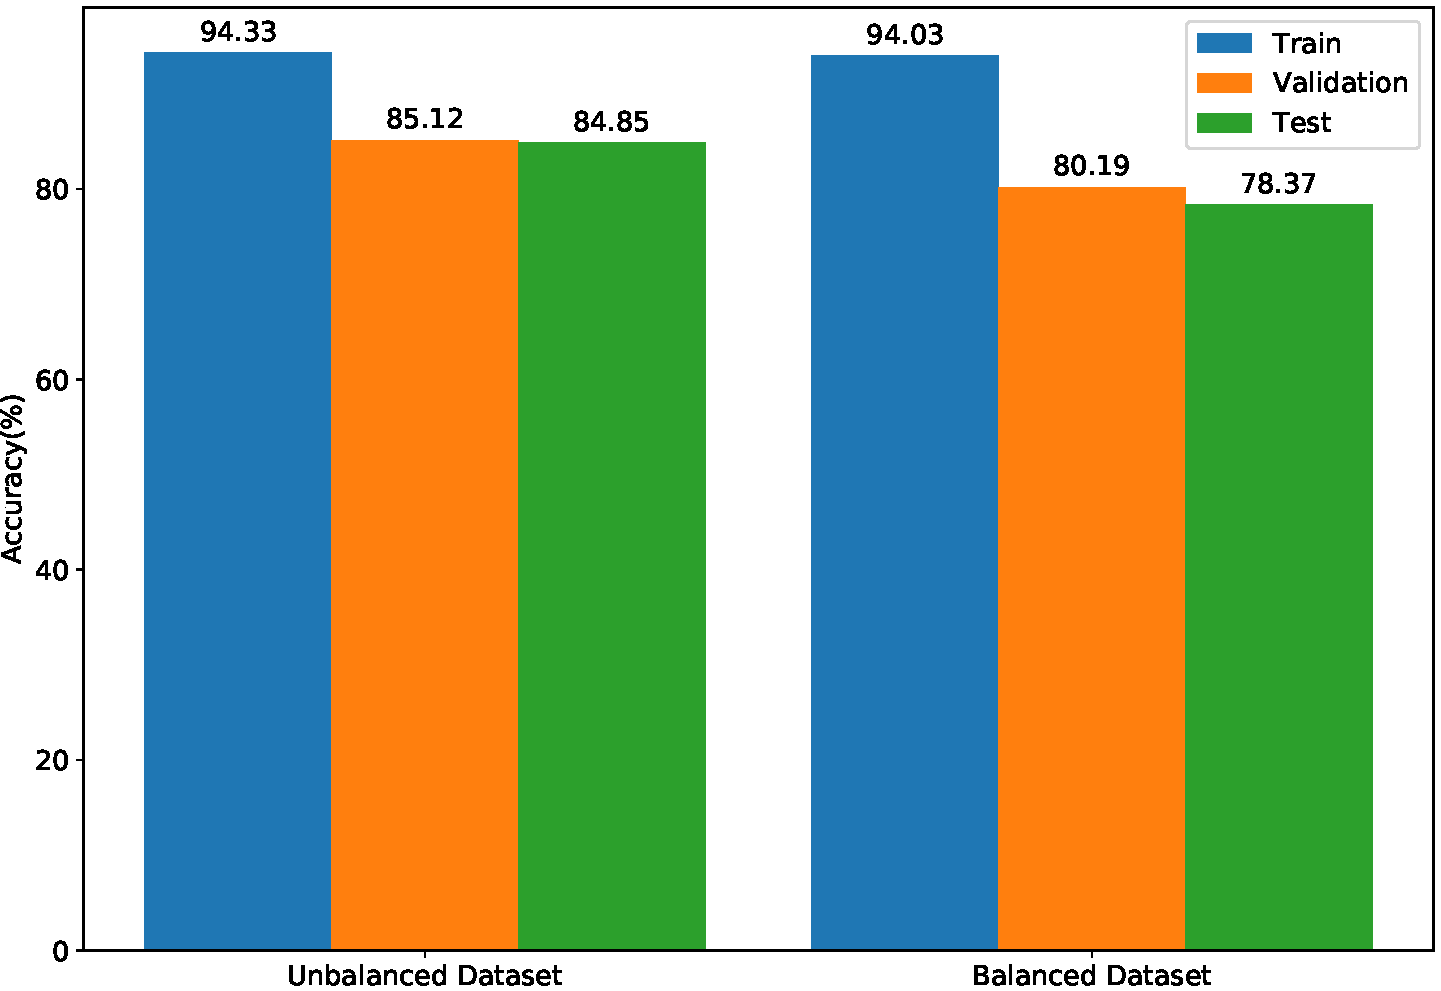
\includegraphics[width=0.9\textwidth]{figs/densenet201_acc_comp.pdf}
        \caption[Comparison of the accuracy of balanced and unbalanced datasets with 20518 samples for the train, validation and test sets using the hyperparameter optimized and fine-tuned DenseNet121 pre-trained model.]{Comparison of the accuracy of balanced and unbalanced datasets with 20518 samples for the train, validation and test sets using the hyperparameter optimized and fine-tuned DenseNet121 pre-trained model. Online data augmentation is turned on using group 1.}
        \label{fig:densenet201_acc_comp}
    \end{figure}
    
    From the results shown, one can hypothesize that reducing undersampling from overrepresented classes, while keeping classes balanced using offline data augmentation would yield better overall accuracy and \ac{BMA} scores. Figure \ref{fig:densenet201_balanced_samples_metrics_comp} shows the influence of different balanced dataset sizes on the \ac{BMA} and accuracy scores. Larger balanced datasets are created by decreasing the undersampling of original samples on overrepresented classes and increasing oversampling through offline data augmentation on underrepresented classes. Furthermore, experiments were made for 10000, 20000, 30000, 40000, 50000, 60000, 70000, and 83432 class balanced datasets, in which the dataset with 83432 samples has no undersampling being applied, meaning that no original samples are discarded. Therefore, each class of the dataset with 83432 samples has 10429 samples because the most overrepresented class in the training set is the melanocytic nevus (NV) with 10429 samples. \par
    
    Considering the results from \autoref{fig:densenet201_balanced_samples_metrics_comp}, it seems that increasing the dataset through offline data augmentation does improve \ac{BMA} and accuracy scores on both the test and validation sets. Furthermore, on the training dataset, the \ac{BMA} scores approximate the accuracy scores, which is to be expected because the training dataset is balanced (recall \Cref{section:metrics}). \par
    
    The \ac{BMA} and accuracy scores are close together on test and validation sets on smaller datasets such as with 10000, 20000, and 30000 samples. However, with larger datasets, the gap between \ac{BMA} and accuracy scores start to increase. This gap is due to an overall increase in the generalization performance of overrepresented classes, while underrepresented classes do not keep improving. This happens because on smaller datasets overrepresented classes are undersampled, but most if not all of the underrepresented classes are already being oversampled. Therefore, performance towards overrepresented classes keeps rising, which greatly influences the accuracy scores, but underrepresented classes keep the same performance, which in turn makes a small impact on \ac{BMA} scores. These results support the notion that past a certain number of synthetically generated samples, oversampling has close to no effect on generalization performance of underrepresented classes. \par
    
    Furthermore, although oversampling the original dataset with class balancing seems to reduce overfitting, one can argue that this is due to the decrease in the undersampling of overrepresented classes, rather than the oversampling process. One can confirm such hypothesis by looking at the discrepancy of the accuracy and \ac{BMA} on larger datassets. \par
    
    It is also clear from the results that synthetic samples do not have the same impact on generalization performance as original samples. For example, the obtained improvements on the \ac{BMA} scores shown in \autoref{fig:densenet201_balanced_samples_metrics_comp} are considerably lower than the ones obtained in \autoref{fig:densenet_variations_20264_comp} in which the dataset is increased with original samples rather than synthetic ones.  \par
    
    \begin{figure}[ht]
        \centering
        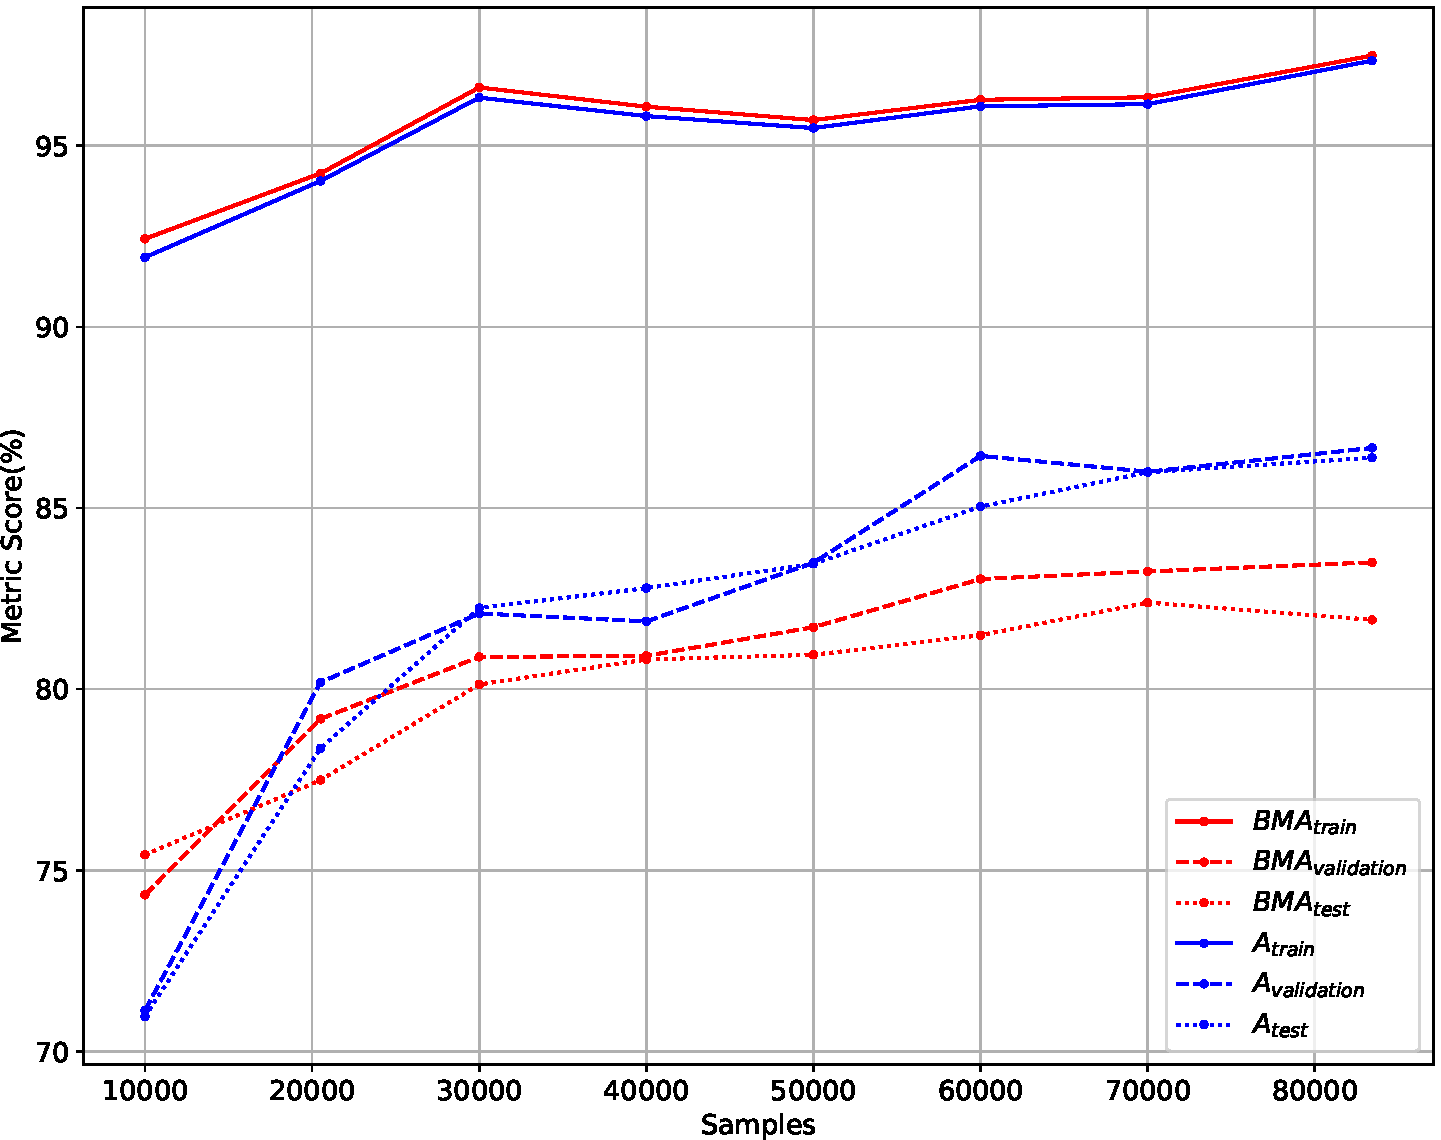
\includegraphics[width=0.9\textwidth]{figs/densenet201_balanced_samples_metrics_comp_proper.pdf}
        \caption[Comparison of train, validation and test \ac{BMA} and accuracy scores for different balanced dataset sizes.]{Comparison of train, validation and test \ac{BMA} and accuracy scores for different balanced dataset sizes using the described oversampling and undersampling techniques. The pre-trained model used is the hyperparameter optimized and fine-tuned DenseNet121. Online data augmentation is turned on using augmentation group 1.}
        \label{fig:densenet201_balanced_samples_metrics_comp}
    \end{figure}

    Finally, the DenseNet121 model trained with online data augmentation (group 1) on the class balanced dataset with 83432 samples is able to attain an accuracy of $86.70\%$ and a \ac{BMA} of $81.5\%$ (see \autoref{fig:densenet201_balanced_samples_metrics_comp}). These results show the remarkable impact of online and offline data augmentation techniques on the generalization performance of the network. This represents a significant improvement from the results obtained in \Cref{section:dataset_impact}, where the model was not using class balanced samples. Presumably, this jump in performance is due to an increase in sample size for classes that are underrepresented on the original dataset. One can confirm such hypothesis by looking at \autoref{fig:82400_balanced_conf_matrix}, which in comparison with \autoref{fig:unbalanced_full_dataset_conf_matrix} shows that the network is more capable of correctly classifying underrepresented classes. \par
    \begin{figure}[ht]
        \centering
        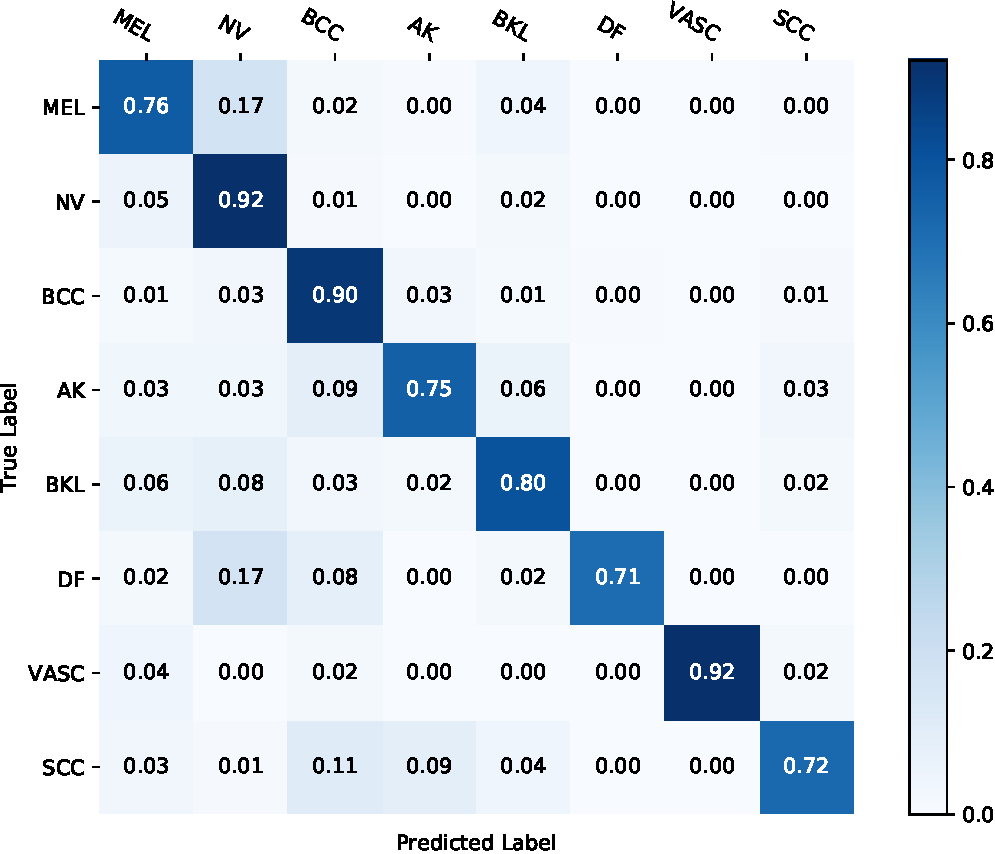
\includegraphics[width=0.7\textwidth]{figs/densenet201_82400_balanced_conf_matrix.pdf}
        \caption{Confusion matrix of the hyperparameter optimized and fine-tuned DenseNet121 pre-trained model, trained with the balanced and oversampled \ac{ISIC} 2019 dataset with 83432 samples. Online data augmentation was turned on during training with augmentation group 1.}
        \label{fig:82400_balanced_conf_matrix}
    \end{figure}
    
\section{Model Ensemble} 
\label{section:ensemble}
    The literature suggests that the most successful approaches towards \ac{ISIC} challenges are those based on an ensemble of classifiers \cite{humanvsisic2018}. Even though this methods might not be practical for real world scenarios due to the added computational requirements, it might be useful to assess what improvements it could bring to the generalization performance of this approach. \par
    
    As seen in \Cref{section:skin_transfer_learning}, in order to properly create an ensemble one must combine different classifiers trained on different conditions (\textit{e.g.}, model architectures, hyperparameters) or with different data (\textit{e.g.} bagging). However, an ensemble of different models pre-trained on ImageNet will be created because in this study different pre-trained models were already studied in \Cref{section:models}. Furthermore, an important aspect to consider is that simply selecting different pre-trained models within the same architecture is not enough because the different variations within a model architecture are just scaled up/down versions of a baseline model. Therefore, averaging the predictions of such models would not significantly increase the overall performance because each model would produce similar results (\textit{e.g.}, VGG16, and VGG19 or EfficienNetB2 and EfficientNetB0). 
    
    Therefore, the choice of the models to use from each architecture in the ensemble is made based on the results from \autoref{fig:pre_trained_model_val_comp}. More specifically, this approach selects the best performing model from each architecture: VGG16, ResNet152, InceptionResNetV2 and EfficientNetB2. The exception to this criteria is the DenseNet, as the chosen model is the DenseNet121 instead of the DenseNet201 (see arguments behind this decision in \Cref{section:dataset_impact}). \par
    
    Furthermore, different combinations between each of these models will be presented in order to attain the best possible performance. For simplification, all models will use the hyperparameters optimized for DenseNet in \Cref{section:hyperparameters}. All the models were trained under the same conditions based on the previous section's results, more specifically:
    \begin{itemize}
        \item An global average pooling layer is introduced at the end of the convolutional base in order to reduce the number of parameters for the classifier;
        \item The original pre-trained model's classifier is replaced by a new classifier composed of one fully-connected layer with 512 neurons which use the ReLU activation function, and one softmax layer with 8 neurons to translate each of the class's probabilities;
        \item Extracting all layer's weights while also fine-tuning these layers, which as shown in \Cref{section:models} yields higher performance since it will continue to optimize parameters relative to the target dataset;
        \item Following the work done by Gessert \textit{et al.} \cite{gessert2018} the Adam optimizer \cite{adam} is used, with $\rho_{1} = 0.9$ and $\rho_{2}=0.999$;
        \item The convolutional base is frozen for the initial 2 epochs with a learning rate of $10^{-3}$. The initial fine-tuning learning rate is $10^{-4}$ but is reduced by a factor of 10 when validation loss stops improving for 8 epochs. Each model trains for a maximum of 100 epochs but early stopping is performed whenever validation loss stops improving for 16 epochs;
        \item For each epoch, all the samples are shuffled before being feed into the network;
        \item Each batch is composed of 8 samples;
        \item Both online and offline data augmentation are used with random crops, rotations, and flips each with a probability of 0.5. Offline data augmentation is used as a class balancing measure and online data augmentation as a method to alleviate overfitting;
        \item For each training process, 3 models are saved: The model that obtained the highest \ac{BMA} on the validation set, the model with the lowest loss on the validation set, and finally the resulting model from the last epoch. However, the performance on the test set is evaluated according to the model which attained the highest \ac{BMA} on the validation set.
    \end{itemize}
    
    \begin{table}[h]
        \centering
        \begin{tabularx}{\textwidth}{|l|X|X|X|}
            \hline
            Approach Name & Pre-trained models & \ac{BMA} & Accuracy \\ \hline
            EfficientNetB2 approach & EfficientNetB2 & $\approx$ 0.820 & $\approx$ 0.851 \\ \hline
            DenseNet121 approach & DenseNet121 & $\approx$ 0.815 & $\approx$ 0.867 \\ \hline
            InceptionResNetV2 approach & InceptionResNetV2 & $\approx$ 0.811 & $\approx$ 0.862 \\ \hline
            ResNet152 approach & ResNet152 & $\approx$ 0.797 & $\approx$ 0.858 \\ \hline
            VGG16 approach & VGG16 & $\approx$ 0.753 & $\approx$ 0.824 \\ \hline
            Ensemble of best 2 models & EfficientNetB2, DenseNet121 & $\approx$ 0.842 & $\approx$ 0.878 \\ \hline
            Ensemble of best 3 models & EfficientNetB2, DenseNet121, InceptionResNetV2 & $\approx$ 0.846 & $\approx$ 0.891 \\ \hline
            Ensemble of best 4 models & EfficientNetB2, DenseNet121, InceptionResNetV2, ResNet152 & $\approx$ 0.841 & $\approx$ 0.894 \\ \hline
            Ensemble of all 5 models & EfficientNetB2, DenseNet121, InceptionResNetV2, ResNet152, VGG16 & $\approx$ 0.836 & $\approx$ 0.893  \\ \hline
        \end{tabularx}
        \caption[\ac{BMA} and Accuracy of different models and ensembles for 8-class classification of skin lesions.]{\ac{BMA} and Accuracy of different models and ensembles for 8-class classification of skin lesions. The Softmax probabilities a ensemble's models are averaged together in order to create each ensemble. All models (including models within ensembles) are fine-tuned and use the best hyperparameters found in \Cref{section:hyperparameters}. The training dataset is composed of 83432 class balanced samples (offline data augmentation) where synthetic samples are created using the augmentation group 1. Online data augmentation is turned on with augmentation group 1 as a measure to reduce overfitting.}
        \label{tables:82400_ensemble}
    \end{table} 

    Results from \autoref{tables:82400_ensemble} show significant improvements of all ensembles over single-model performance on both \ac{BMA} and accuracy, with the ensemble of the best 3 models being the best performing one reaching near 90\% accuracy. Presumably, all the ensembles have superior performance to single models, because one is averaging predictions across models with significantly different architectures. This produces significant variations within the softmax probabilities, which when averaged produce better generalization performance. \par
    
    One can also observe that ensembling the most amount models is not necessarily the best approach. For example, the ensemble of the best 4 and the ensemble of 5 yields significantly worse performance than the ensemble of the best 3. This can be attributed to the discrepancy in the performance of VGG16 and ResNet152 concerning the rest of the models (EfficientNetB2, DenseNet121, InceptionResNetV2), which as a consequence of the averaging scheme brings the performance metrics down. However, the models composing the ensemble of the best 3 all have similar performance, which makes them good candidates for an ensemble with an averaging scheme. Moreover, one can assume that if more models were available with similar performance to the EfficientNetB2, DenseNet121, and InceptionResNetV2 then it would result in better \ac{BMA} and accuracy scores. 
    
    Finally, the confusion matrix of the ensemble of the best 3 models is shown in \autoref{fig:densenet201_best_ensembe_3}. Results show that overall every class has a slightly better performance when compared to the single-model performance of DenseNet121 in \autoref{fig:82400_balanced_conf_matrix}. This performance increase also reflects on the \ac{BMA} and accuracy values, which become 0.846 and 0.891, respectively.\par
    
    \begin{figure}[ht]
        \centering
        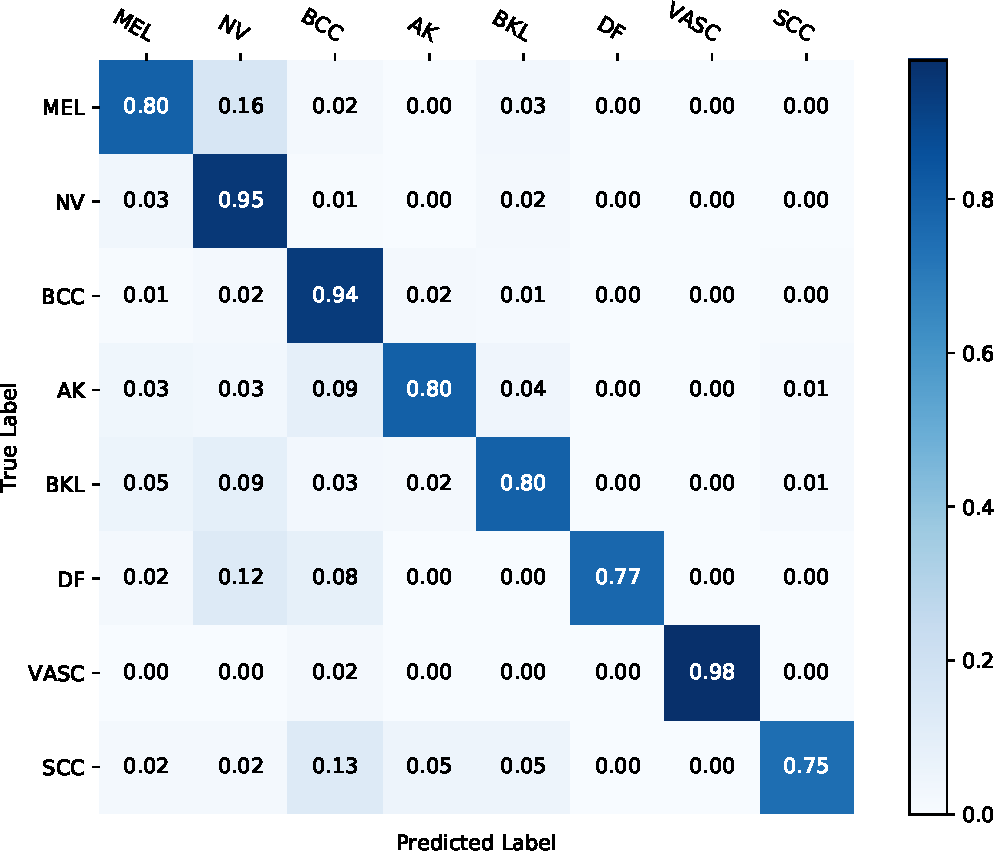
\includegraphics[width=0.7\textwidth]{figs/densenet201_best_ensembe_3.pdf}
        \caption[Confusion matrix of the ensemble composed with the best 3 pre-trained models.]{Confusion matrix of the ensemble composed with the best 3 pre-trained models, namely DenseNet121, EfficientNetB2 and InceptionResNetV2. Each model is trained with 83432 balanced samples with the best hyperparameters obtained in \Cref{section:hyperparameters}. Online data augmentation is turned on.}
        \label{fig:densenet201_best_ensembe_3}
    \end{figure}



\section{Out of Training Distribution Detection} \label{section:outdist}
    The presented models in \Cref{section:balance} and \Cref{section:ensemble} show that deep \ac{CNN}s can be effective predictors on the task of skin lesion classification. However, no out-of-distribution detection is being performed to identify "unknown" samples. In other words, the model is unaware of whether a test sample is part of the original train data distribution (\textit{i.e.}, the original 8 classes) or not. As presented in \Cref{chapter:sota}, in the \ac{ISIC} 2019 challenge, there is not a single way of identifying out-of-distribution samples, consequently resulting in a multitude of methodologies being employed by different authors. As a means to compare such methods, this work will explore 3 of them, namely:
    
    \begin{itemize}
        \item Following the submission by Zhou \textit{et al.} \cite{isic2019second}, experiments will be made with different top-1 softmax probability thresholds;
        \item The \ac{ODIN} \cite{odin} will be integrated within the single-model approach, following Wang's submission towards the \ac{ISIC} 2019 \cite{Wang};
        \item Finally, like Gessert \textit{et al.} \cite{isic2019first} (\ac{ISIC} 2019 winner), results of out-of-distribution detection will be presented by training a model with an additional outlier class, composed of additional samples.
    \end{itemize}
    
    A benchmark has been set to test and compare these 3 approaches, more specifically:
    \begin{itemize}
        \item For simplicity of the results, the single best model approach towards 8 class classification, namely the hyperparameter tuned DenseNet121 model, will be used instead of the ensemble presented at \cref{section:ensemble};
        \item An global average pooling layer is introduced at the end of the convolutional base in order to reduce the number of parameters for the classifier;
        \item The original pre-trained model's classifier is replaced by a new classifier composed of one fully-connected layer with 512 neurons which use the ReLU activation function, and one softmax layer with either 8 or 9 neurons to translate each of the class's probabilities;
        \item For the transfer learning approach, all the layer's parameters from the convolutional base of the pre-trained model are extracted and fine-tuned, which yields the best performance for this specific dataset (see the results presented in \Cref{section:models});
        \item Following the work done by Gessert \textit{et al.} \cite{gessert2018} the Adam optimizer \cite{adam} is used, with $\rho_{1} = 0.9$ and $\rho_{2}=0.999$;
        \item The convolutional base is frozen for the initial 2 epochs with a learning rate of $10^{-3}$. The initial fine-tuning learning rate is $10^{-4}$ but is reduced by a factor of 10 when validation loss stops improving for 8 epochs. Each model trains for a maximum of 100 epochs but early stopping is performed whenever validation loss stops improving for 16 epochs;
        \item For each epoch, all the samples are shuffled before being feed into the network;
        \item Each batch is composed of 8 samples.
        \item Online and offline data augmentation is used, with random crops, rotations, and flips each with a probability of 0.5 (augmentation group 1). Offline data augmentation is used a class balancing measure and online data augmentation as a method to alleviate overfitting;
        \item For each training process, 3 models are saved: The model that obtained the highest \ac{BMA} on the validation set, the model with the lowest loss on the validation set, and finally the resulting model from the last epoch. However, the performance on the test set is evaluated according to the model which attained the highest \ac{BMA} on the validation set.
    \end{itemize}
    
    \subsection{Softmax Threshold}
        Multi-class classification problems using deep neural networks often use a softmax layer at the last layer of the neural network classifier. The softmax probabilities of a softmax layer always add up to 1 and are spread across all classes with non-zero values. As such, the network will presumably try to optimize softmax probabilities by maximizing the softmax of the ground truth class and minimizing the probabilities for other classes. Even though the softmax predictions of an out-of-distribution sample in an 8-class model will add up to 1, one can make the assumption that the highest score will be lower than an in-distribution sample because the model will likely not be confident of its predictions. \par
        
        Therefore, a threshold will be imposed on the softmax so that if the top softmax probability is lower than that threshold, then the sample will be labeled as "unknown", or more formally known as an out-of-distribution sample. However, there is no clear threshold value that will benefit the model the most. The experiments shown in \autoref{fig:densenet121_threshold_comp} suggest that low thresholds have close to no impact on the classification of the out-of-distribution samples, while high thresholds negatively impact the model performance. 
        \begin{figure}[ht]
            \centering
            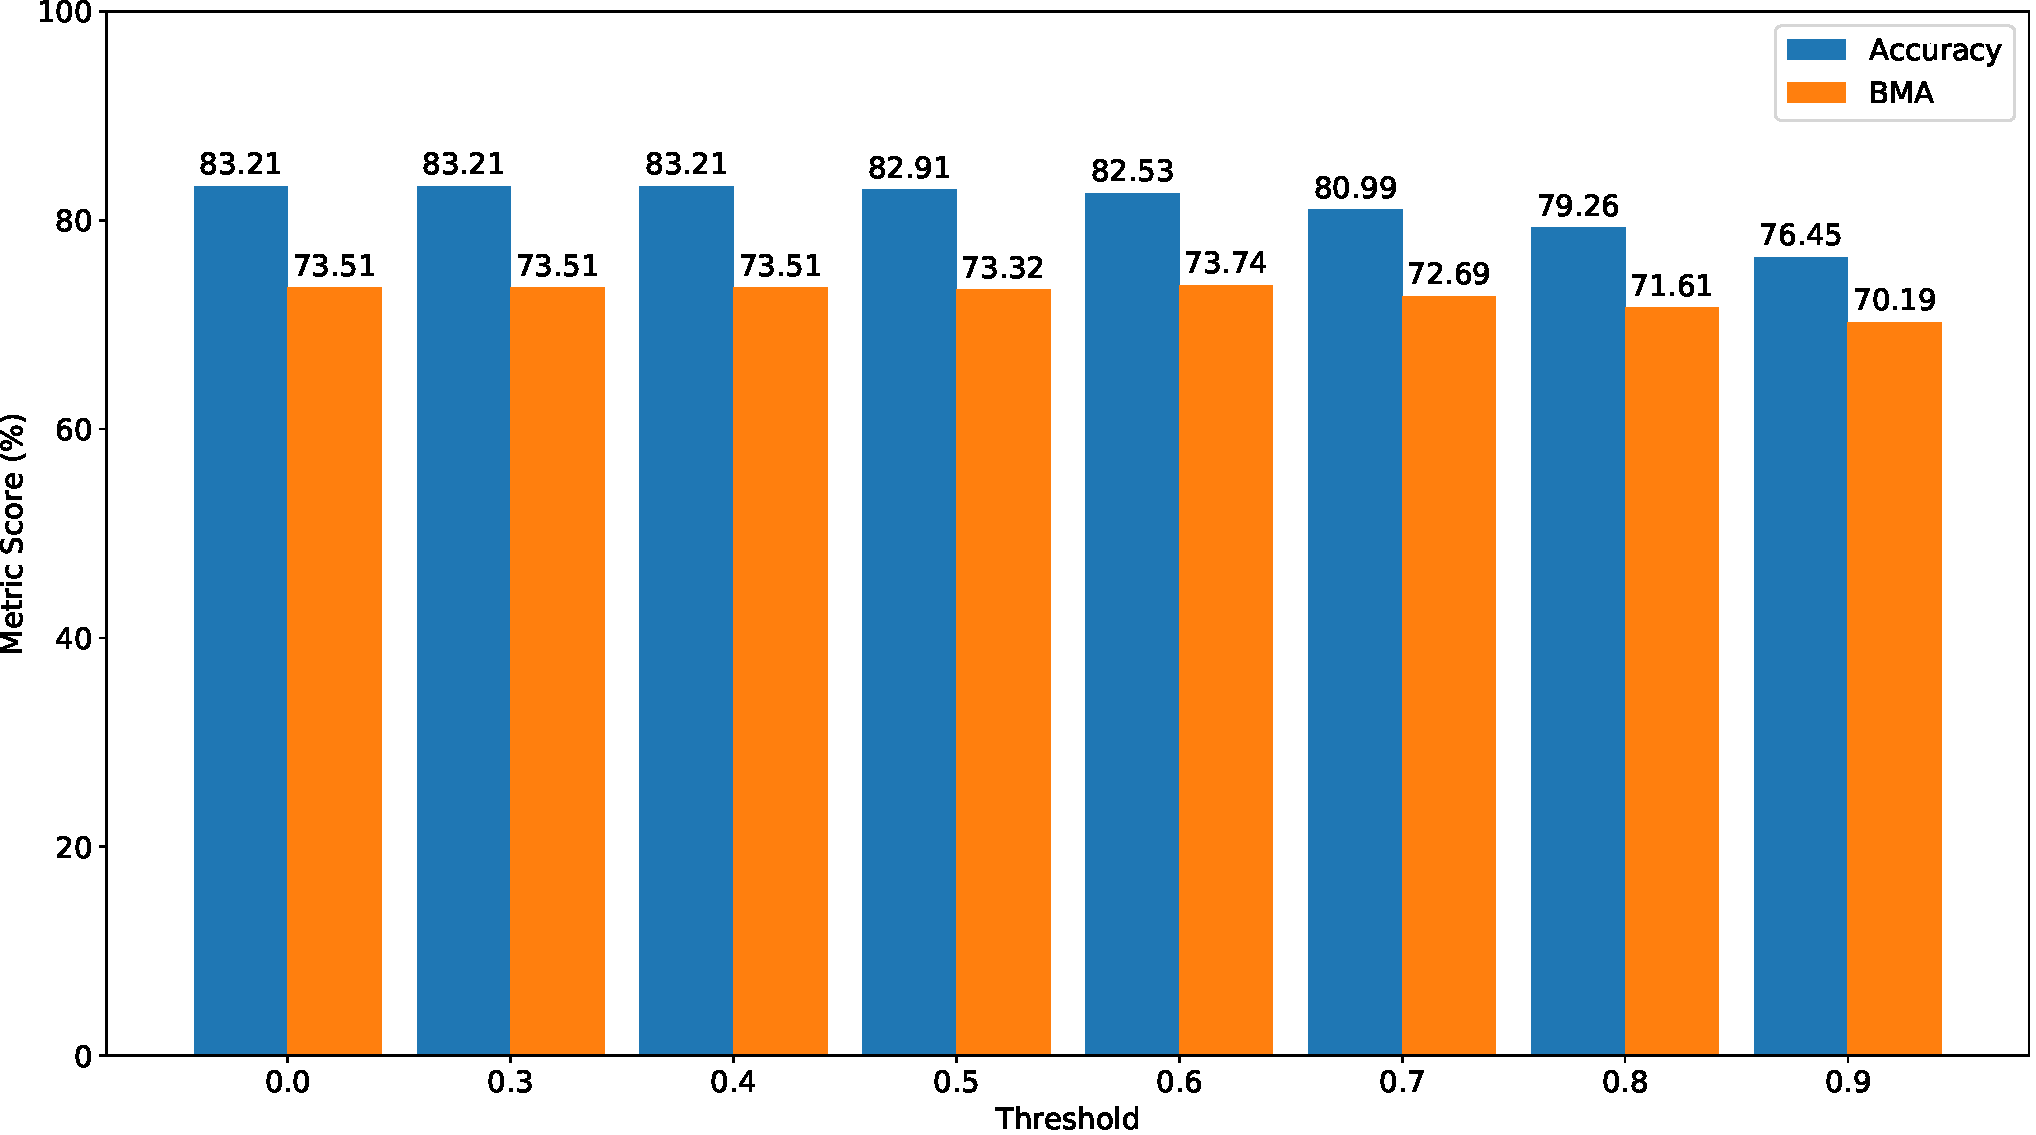
\includegraphics[width=\textwidth]{figs/densenet121_threshold_comp.pdf}
            \caption{Comparison of different top-1 softmax threshold values for the detection of out of training distribution samples from the test set.}
            \label{fig:densenet121_threshold_comp}
        \end{figure}
        
        Considering the results, low threshold values having no impact stem from the fact that the DenseNet model often outputs high softmax scores towards a specific class (see the examples from \autoref{fig:softmax_examples}). This is an expected attribute of these types of deep learning models because they were optimized for 8 classes as opposed to 9, which means that they will try to maximize softmax scores towards one of the 8 classes rather than considering that a sample might not be part of the initial 8 class distribution of the training dataset. \par
        
        This property also reflects in the results of higher thresholds, because such thresholds start negatively impacting correctly classified samples from other classes as seen by the confusion matrix in \autoref{fig:densenet121_conf_matrix_thresh_0_7}. These results show a bright contrast with the ones obtained by Hendricks \textit{et al.} \cite{Hendrycks2019} for his baseline approach towards out-of-distribution detection (recall \Cref{section:out_of_distribution}). However, one should take into consideration that the in-distribution dataset used by them is far different from the out-of-distribution samples. More specifically, they presented results with  \ac{MNIST} \cite{LeCun1998} as an in-distribution dataset and out-of-distribution datasets such as Gaussian Noise, uniform noise and black and white CIFAR-10 \cite{Krizhevskya} samples. Unfortunately, for the problem of skin lesion classification in- and out-of-distribution samples can be quite similar which makes this approach sub-optimal.
        
        \begin{figure}[ht]
            \centering
            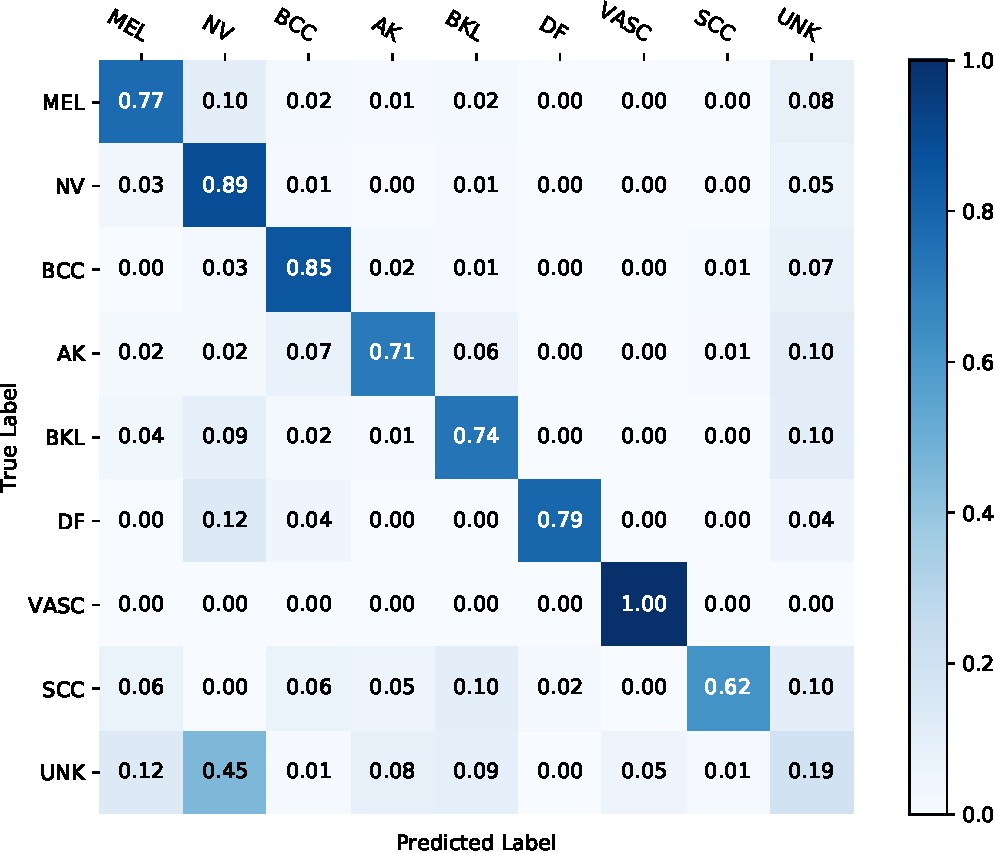
\includegraphics[width=0.7\textwidth]{figs/densenet121_conf_matrix_thresh_0_7.pdf}
            \caption[Confusion matrix of the test set predictions on the hyperparameter tuned DenseNet121 trained with 8 classes where out of distribution samples are identified using a top-1 softmax threshold of 0.7.]{Confusion matrix of the predictions of the test set containing out of training distribution samples. The used model is the hyperparameter tuned DenseNet121 trained with 83432 class balanced samples from 8 different classes, and online data augmentation is performed with group 1 as a method to reduce overfitting. Out of distribution samples (\textit{i.e.}, "unknown" samples) are identified using a top-1 softmax threshold of 0.7.}
            \label{fig:densenet121_conf_matrix_thresh_0_7}
        \end{figure}

        
    \subsection{\ac{ODIN}}
        As demonstrated in \Cref{section:out_of_distribution}, there are 3 parameters within the \ac{ODIN} that need tuning, namely: the temperature scaling $T$, the perturbation magnitude $\varepsilon$ and the threshold $\sigma$. However, as this tuning procedure has already been done by Hsin-Wei Wang Wang \cite{Wang} for the same dataset (\ac{ISIC} 2019 challenge dataset), it has been decided to not tune these parameters, but to rather use the ones already tuned by this author. More specifically, $T = 2$, $\varepsilon = 0.0002$ and $\sigma = 0.90385$. \par
        
        Results with this method present an accuracy of 69.08\% and a \ac{BMA} of 65.35\% over the test set. As shown in the confusion matrix of \autoref{fig:densenet121_conf_matrix_odin}, it is clear that \ac{ODIN} is not performing well enough as predictions towards the unknown class are evenly distributed across the 9 classes. It is hypothesized that ODIN is not a good option for out-of-distribution detection in skin lesion classification, because in and out of distribution samples are very similar to each other. This means that techniques like temperature scaling and adding small perturbations to the inputs have a small impact on the classification results. \par 
        \begin{figure}[ht]
            \centering
            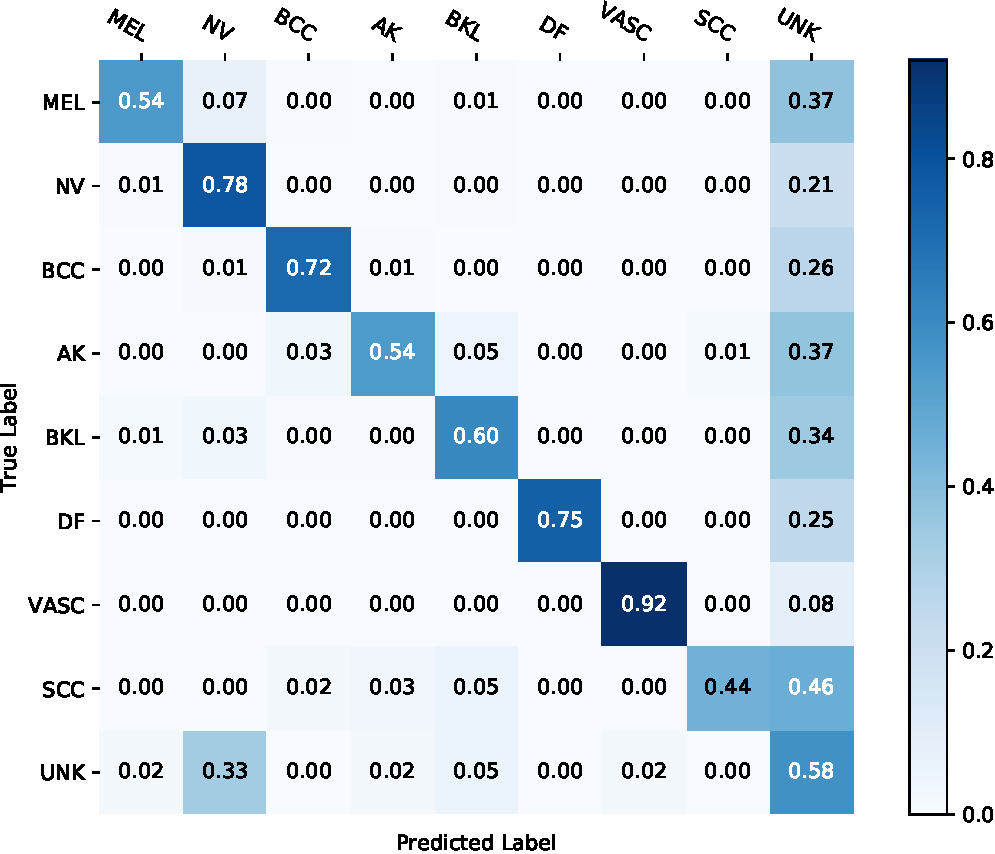
\includegraphics[width=0.7\textwidth]{figs/densenet121_conf_matrix_odin.pdf}
            \caption[Confusion matrix of the test set predictions on the hyperparameter tuned DenseNet121 trained with 8 classes where out of distribution samples are identified using the \ac{ODIN} detector.]{Confusion matrix of the predictions of the test set containing out of training distribution samples. The used model is the hyperparameter tuned DenseNet121 trained with 83432 class balanced samples from 8 different classes, and online data augmentation is performed with group 1 as a method to reduce overfitting. Out of distribution samples (\textit{i.e.}, "unknown" samples) are identified using \ac{ODIN} \cite{odin}}
            \label{fig:densenet121_conf_matrix_odin}
        \end{figure}
        
        These results contrast the results obtained by Liang \textit{et al.} \cite{odin}, where the in and the out-of-distribution samples were quite different from each other. More specifically, in distribution images belonged to the CIFAR-10 \cite{Krizhevskya} which consists of 60000 images in 10 classes and the out-of-distribution samples were either from a uniform noise distribution, a Gaussian noise distribution, the Tiny ImageNet dataset (a subset of the ImageNet dataset \cite{Deng2010}) which is composed of 200 classes, or finally from the LSUN dataset \cite{Yu2015} which is composed of 30 classes (10 scene categories and 20 object categories). From this, one can assume that \ac{ODIN} only works well when the training dataset is far different from the out of distribution samples. \par 
        
    \subsection{Outlier Class}
        From the results so far, it is evident that only using the softmax probabilities is not enough to determine whether a sample belongs to the training dataset. As such, the final approach towards out of distribution detection is to re-train the original DenseNet121 model with a 9th class with the out of distribution data described in \Cref{chapter:environment}. \par
        
        Samples are split into train, validation, and test in a stratified way just like in the previous experiments (see \Cref{section:split}). This means that very few samples are used to train, validate, and test this class. Therefore, to alleviate this problem, the outlier class is oversampled through the data augmentation group 1 so that all classes are balanced (just like the final approach defined in \Cref{section:data}). In practice, this means that a DenseNet121 is trained with 93861 samples (most of them synthetic). \par
        
        \begin{figure}[ht]
            \centering
            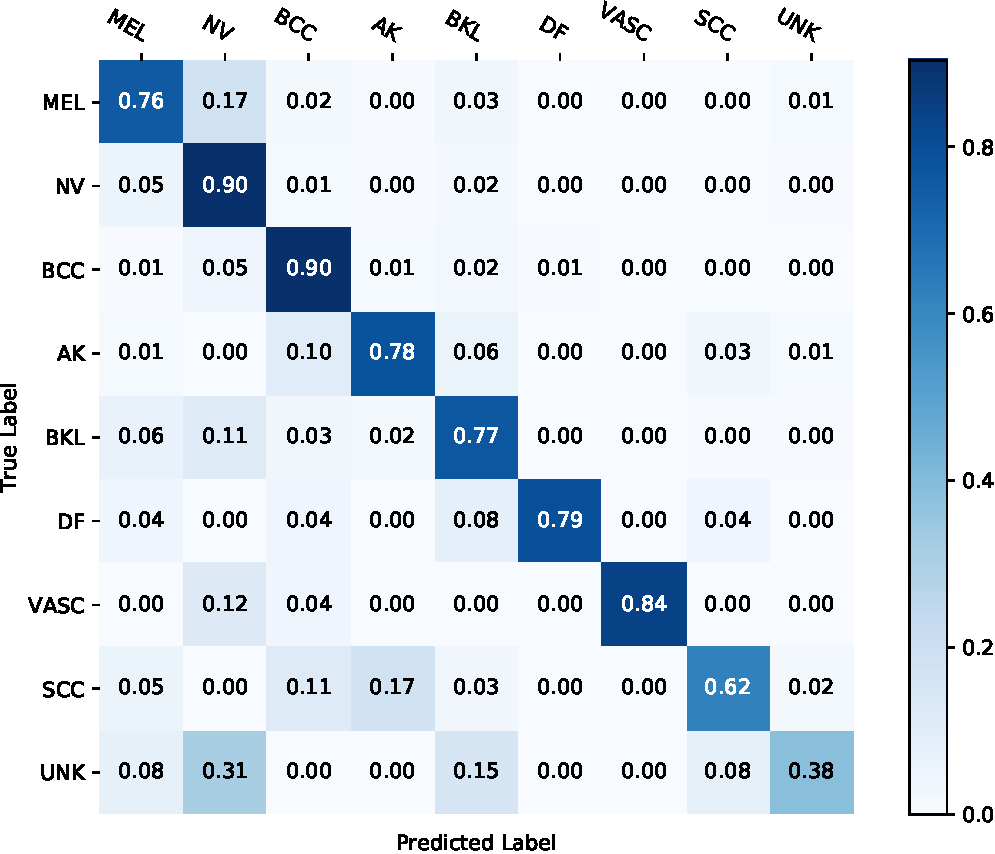
\includegraphics[width=0.7\textwidth]{figs/densenet121_conf_matrix_unknown_train.pdf}
            \caption[Confusion matrix of the test set predictions on the hyperparameter tuned DenseNet121 trained with in and out of distribution samples]{Confusion matrix of the test set predictions on the hyperparameter tuned DenseNet121 trained with 93861 samples class balanced samples from 9 different classes. The 9th class is composed of the out of distribution data described in \Cref{chapter:environment}. Online data augmentation is performed with the group 1 as a method to reduce overfitting.}
            \label{fig:densenet121_conf_matrix_9thclass}
        \end{figure}
        
        As shown in the confusion matrix in \autoref{fig:densenet121_conf_matrix_9thclass}, results are considerably better than the previous approaches with an overall accuracy of 84.72\% and a \ac{BMA} of 74.98\%. However, it is still very apparent that the "unknown" class has significantly lower performance than the rest of the classes. These findings can be attributed to the small amount of rather heterogeneous samples in this class used to train the model. One can also observe that there are a lot of out-of-distribution samples (UNK) that are being classified as Melanocytic Nevus (NV) and then again one can speculate that this might be due to a lack of data for the "unknown" class. \par
        
    \subsection{Approach Comparison}
    Finally, these 3 approaches are compared in \autoref{tables:unknown_comp}, with respect to the test \ac{BMA} and accuracy scores. It is evident from the results that training an outlier class outperforms both softmax thresholding and the \ac{ODIN} method. These findings corroborate the results attained in the literature, specifically, Hsin-Wei Wang reported that the \ac{ODIN} classifier performed poorly due to an insignificant difference between in and out of distribution samples \cite{Wang}. In contrast, approaches such as the one done by Gessert \textit{et al.} \cite{isic2019first} attained one of the best results in 9-class classification, presumably because of the availability of a big in-house dataset used to train an outlier class composed of out of distribution samples (in-distribution being the original 8 classes). As such, more effort should be put into gathering a bigger set of "unknown" samples. \par
    \begin{table}[h]
        \centering
        \begin{tabularx}{\textwidth}{|l|X|X|}
            \hline
            Out-of-distribution method & \ac{BMA} & Accuracy \\ \hline
            Softmax threshold (0.7) & 0.721 & 0.823 \\ \hline
            \ac{ODIN} & 0.654 & 0.691 \\ \hline
            Outlier class & 0.750 & 0.847 \\ \hline
        \end{tabularx}
        \caption{Comparison of \ac{BMA} and accuracy scores on the test set for the different methodologies to detect out of training distribution samples.}
        \label{tables:unknown_comp}
    \end{table} 
    
    However, it is important to point out some limitations of the outlier class approach. Specifically, there are very few "unknown" samples within the test set, which might be an indicator that the results might be biased. Furthermore, a good portion of the samples from the "unknown" test set belong to "Lentigo NOS". This might also be negatively impacting the training process for the outlier class approach because the most effective way of minimizing the loss within the "unknown" class is by correctly classifying "Lentigo NOS" samples. Moreover, the test set will have more "Lentigo NOS" samples than the rest of the classes which can also be biasing the test set results. \par
    
\section{Results Discussion} 
\label{section:discussion}
    
    Finally, one can now compare the different methods employed throughout this work in \autoref{tables:approach_evoution}. Planned experiments in \Cref{section:balance} corroborated the importance of dataset size for deep neural networks, which significantly improved the performance of the model in comparison to the DenseNet201 employed in \Cref{chapter:experiments}. However, sufficient labeled data for skin lesions is hard to come by, which highlights the importance of data augmentation. The presented comparisons show that simple data augmentation techniques can significantly improve generalization performance through offline data augmentation as a class balancing measure. Furthermore, while online data augmentation proved to be an excellent approach to reduce overfitting, offline data augmentation has a big impact on the generalization performance of underrepresented classes. \par
    
    \begin{table}[h]
        \centering
        \begin{tabularx}{\textwidth}{|l|X|X|}
            \hline
            Approach Step & \ac{BMA} & Accuracy \\ \hline
            Pre-trained model choice (see \Cref{section:models}) & $\approx$ 0.579 & $\approx$ 0.746 \\ \hline
            Hyperparameter tuned model (see \Cref{section:hyperparameters})& $\approx$ 0.585 & $\approx$ 0.754 \\ \hline
            Full dataset model without online DA (see \Cref{section:dg_impact})& $\approx$ 0.636 & $\approx$ 0.799 \\ \hline
            Full dataset model with online DA (see \Cref{section:dg_impact})& $\approx$ 0.769 & $\approx$ 0.849 \\ \hline
            Class balanced model (see \Cref{section:class_bal_impact}) & $\approx$ 0.815 & $\approx$ 0.867 \\ \hline
            Ensemble of 3 models (see \Cref{section:ensemble}) & $\approx$ 0.846 & $\approx$ 0.891 \\ \hline
            Model with out-of-distribution detection (see \Cref{section:outdist}) & $\approx$ 0.750 & $\approx$ 0.847 \\ \hline
        \end{tabularx}
        \caption{\ac{BMA} and accuracy on the test set for the different models created throughout this work.}
        \label{tables:approach_evoution}
    \end{table} 
    
    This study confirms that ensemble learning can further improve the results by using different \ac{CNN} architectures. Experimentation also underlines the importance of choosing the best models for the ensemble, otherwise, it will result in a decrease in performance as a consequence of the averaging scheme. However, one should attain whether it is worth to make such an approach for a practical application of these classifiers. For example, if one were to use the best model ensemble, namely, the 3 model ensemble with DenseNet121, InceptionResNetV2, and EfficientNetB2, then one could expect a performance increase of 3\% (see \autoref{tables:approach_evoution}), but it would require approximately 3 times as much time to predict the class label for all the models, which might become a limiting factor when deploying this classifier into a production environment. Therefore, such an approach is useful for benchmark challenges, but it could be impractical for real-world usage. \par
    
    The presented approach achieves competitive results in the \ac{ISIC} 2019 challenge without the need for additional external data in the original 8 classes. It outperforms the state-of-the-art approaches for 8-class classification on both single-model performance and multi-model performance through ensembling (see \autoref{tables:results_comparisson}). Results from 9-class classification show a significant decrease in both \ac{BMA} and accuracy scores in comparison with 8-class classification due to the underwhelming results of the out-of-distribution detection.  \par
    
    \begin{table}[h]
        \centering
        \begin{tabularx}{\textwidth}{|l|X|X|X|X|}
            \hline
            \multirow{2}{*}{Approach} & \multicolumn{2}{l|}{In distribution (8 Classes)} & \multicolumn{2}{l|}{Out of distribution (9 Classes)} \\ \cline{2-5} &                         $BMA_{test}$ & $A_{test}$ & $BMA_{test}$ & $A_{test}$ \\ \hline
            \textbf{3 Model Ensemble} &                         0.846 & 0.891 & 0.775    &  0.858     \\ \hline
            \textbf{DenseNet121} &                              0.815     & 0.867     & 0.750    & 0.847     \\ \hline
            Gessert \textit{et al.} \cite{isic2019first} &        0.725 & NA     & 0.636 & NA     \\ \hline
            Zhou \textit{et al.} \cite{isic2019second} &        0.753 & NA     & 0.607 & NA     \\ \hline
            Hsin-Wei Wang \cite{Wang} &                0.828 & NA     & 0.505 & NA     \\ \hline
        \end{tabularx}
        \caption[Approach comparison with state-of-the-art approaches on 8- and 9-class classification for the \ac{ISIC} 2019.] {Approach comparison with state-of-the-art approaches on 8- and 9-class classification for the \ac{ISIC} 2019. The proposed approaches are highlighted in bold, namely the "3 Model Ensemble" and the "DenseNet121". The in distribution models (8 classes) are trained with 83432 class balanced samples and the out of distribution models (9 classes) are trained with 93861 class balanced samples, where the 9th class is composed of samples from a different distribution of the original 8 (see \autoref{subsection:unknown}). The approaches from Gessert \textit{et al.} \cite{isic2019first}, Zhou \textit{et al.}, and Hsin-Wei Wang \cite{Wang} are ensembles because it is their best performing models. For a detailed single-model performance of these approaches, relate to their original papers.}
        \label{tables:results_comparisson}
    \end{table} 
    
    The obtained results for 8-class classification of skin lesions in the \ac{ISIC} 2019 dataset, resonate the extensive experimentation done throughout this work, that leads to a systematically better performing model step-by-step. However, some limitations are still present, more specifically, our approach for the "unknown" class was unable to attain good generalization performance, with the highest performing method being the outlier class. This is a fairly limited approach in the sense that one does not know the real-world distribution of this class. Even though other strategies such as softmax thresholding and the \ac{ODIN} were experimented with, those methods proved to be very ineffective in skin lesion diagnosis. \par
    
    Even though the presented results are superior to the state-of-the-art (Gessert \textit{et al.} \cite{isic2019first}) on 9-class classification, it should be noted that the test set used to compute the \ac{BMA} and accuracy for the 9-class classification in this approach was part of the unknown dataset gathered from the \ac{ISIC} archive (see \autoref{subsection:unknown}), rather than the 9-class test set originally used to compare different approaches on \ac{ISIC} 2019. This is the case because the \ac{ISIC} organization does not provide the ground truth data related to the \ac{ISIC} 2019 challenge test data. Furthermore, they do not allow any new submissions towards this challenge leaderboard, in order to compute this approach's metrics. \par